\documentclass{beamer}
%\usetheme{default}
\usetheme{Madrid}
\setbeamertemplate{navigation symbols}{}
\def\mathfamilydefault{\rmdefault}
\usepackage{bm}
\usepackage{float}
\usepackage{subfigure}
\usepackage{multirow}

\newcommand{\hide}[1]{} %hide
\newcommand{\tr}[1]{\textcolor{red}{#1}} %red text
\newcommand{\tb}[1]{\textcolor{blue}{#1}} %blue text
\newcommand{\tg}[1]{\textcolor{green}{#1}} %green text
\newcommand{\beq}[1]{\vspace{-0.02in}\begin{equation}#1\end{equation}\vspace{-0.02in}}
\newcommand{\beqn}[1]{\vspace{-0.03in}\begin{eqnarray}#1\end{eqnarray}\vspace{-0.03in}}
\newcommand{\beal}[1]{\vspace{-0.03in}\begin{align}#1\end{align}\vspace{-0.03in}}
\newcommand{\besp}[1]{\begin{split}#1\end{split}}


\begin{document}


\title{Deep Learning}
\author{Jie Tang}
\date{2015}

\begin{frame}
\titlepage
\end{frame}


\begin{frame}
  \frametitle{Contents}
  \tableofcontents
\end{frame}

\section{Introduction}

\begin{frame}
  \frametitle{Contents}
  \tableofcontents[currentsection]
\end{frame}

\begin{frame}
\frametitle{AlphaGo}
\begin{itemize}
\item AlphaGo Vs. Lee Sedol 9-Dan: 4:1
\begin{figure}
      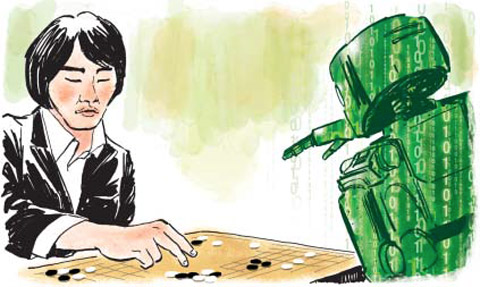
\includegraphics[width=0.8\textwidth]{figs/alphago0.png}
\end{figure}
\item How does it work? 
\end{itemize}
\end{frame}

\begin{frame}
\frametitle{AlphaGo}
\begin{itemize}
\item Core problem: Learn $\mathbf{P(}$\textbf{next action}$ | $\textbf{current state}$\mathbf{)}$
\begin{figure}
      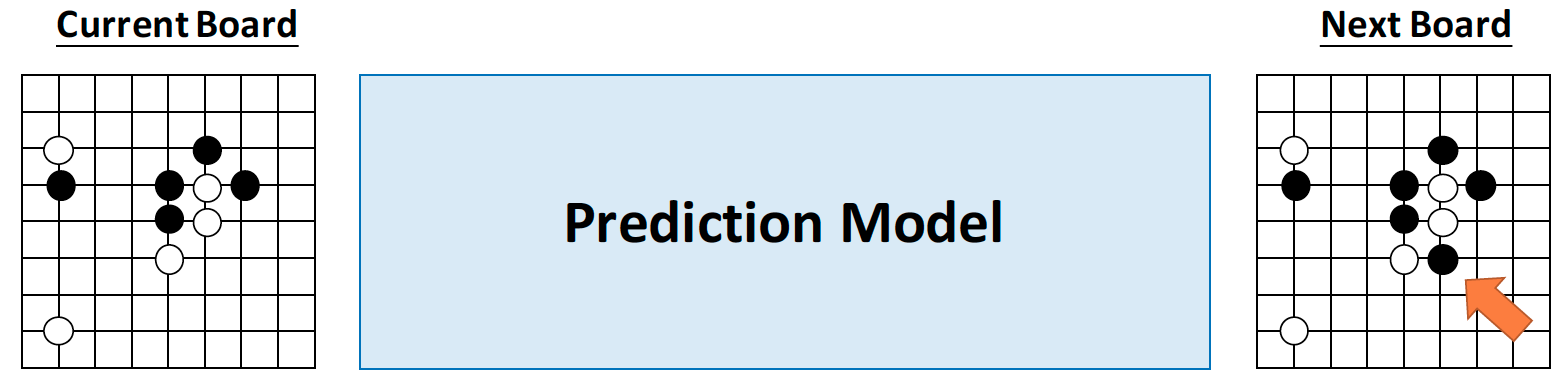
\includegraphics[width=0.9\textwidth]{figs/alphago1.png}
\end{figure}
\item Data: Online Go experts (5-9 dan) 160K games, 30M board positions.
\end{itemize}
\end{frame}


\begin{frame}
\frametitle{AlphaGo}
\begin{itemize}
\item Core problem: Learn $\mathbf{P(}$\textbf{next action}$ | $\textbf{current state}$\mathbf{)}$
\begin{figure}
      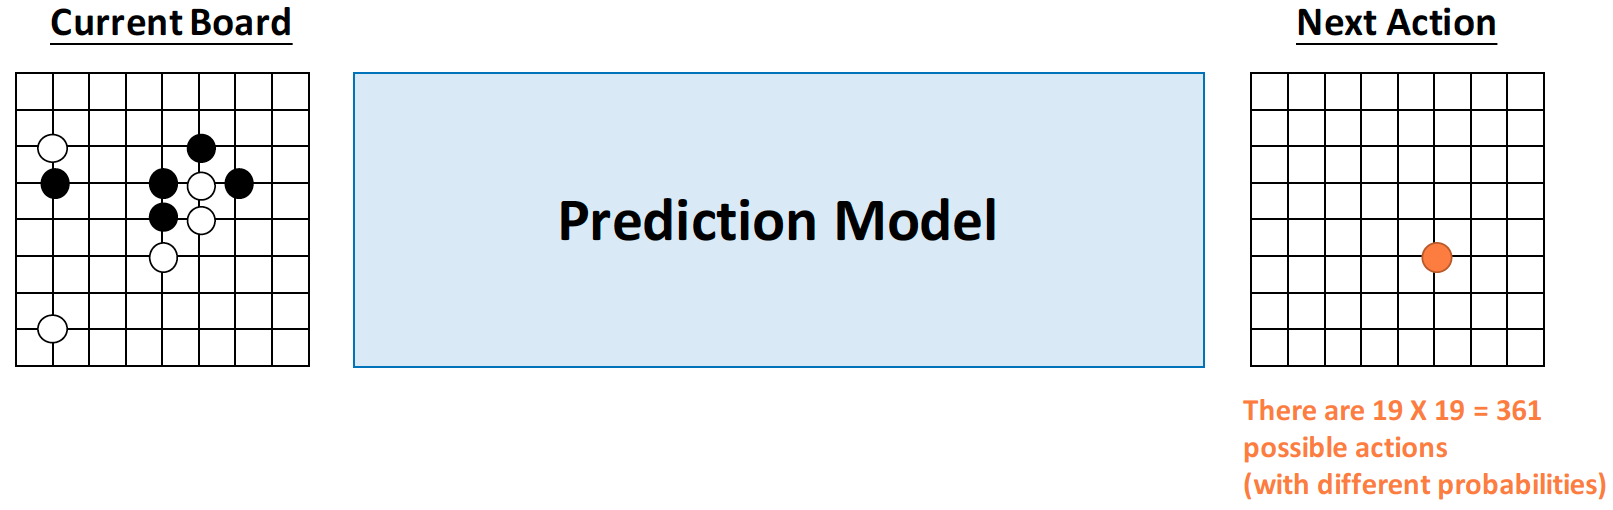
\includegraphics[width=0.9\textwidth]{figs/alphago2.png}
\end{figure}
\end{itemize}
\end{frame}

\begin{frame}
\frametitle{AlphaGo}
\begin{itemize}
\item Core problem: Learn $\mathbf{P(}$\textbf{next action}$ | $\textbf{current state}$\mathbf{)}$
\begin{figure}
      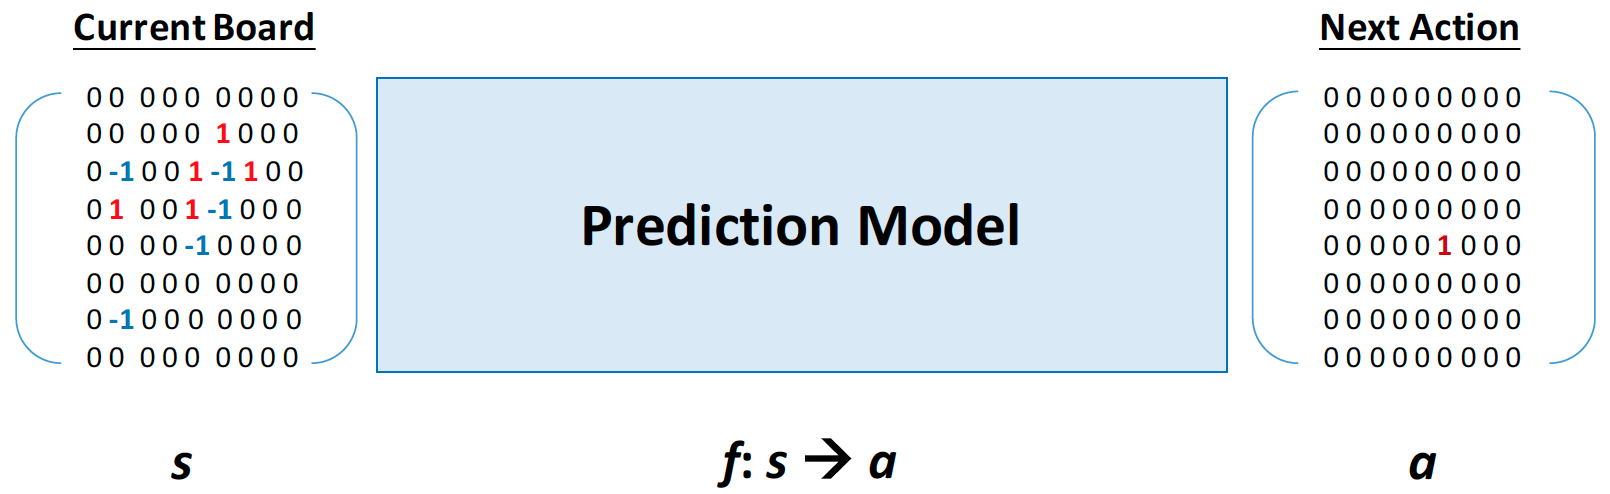
\includegraphics[width=0.9\textwidth]{figs/alphago3.png}
\end{figure}
\end{itemize}
\end{frame}

\begin{frame}
\frametitle{AlphaGo}
\begin{itemize}
\item Core problem: Learn $\mathbf{P(}$\textbf{next action}$ | $\textbf{current state}$\mathbf{)}$
\begin{figure}
      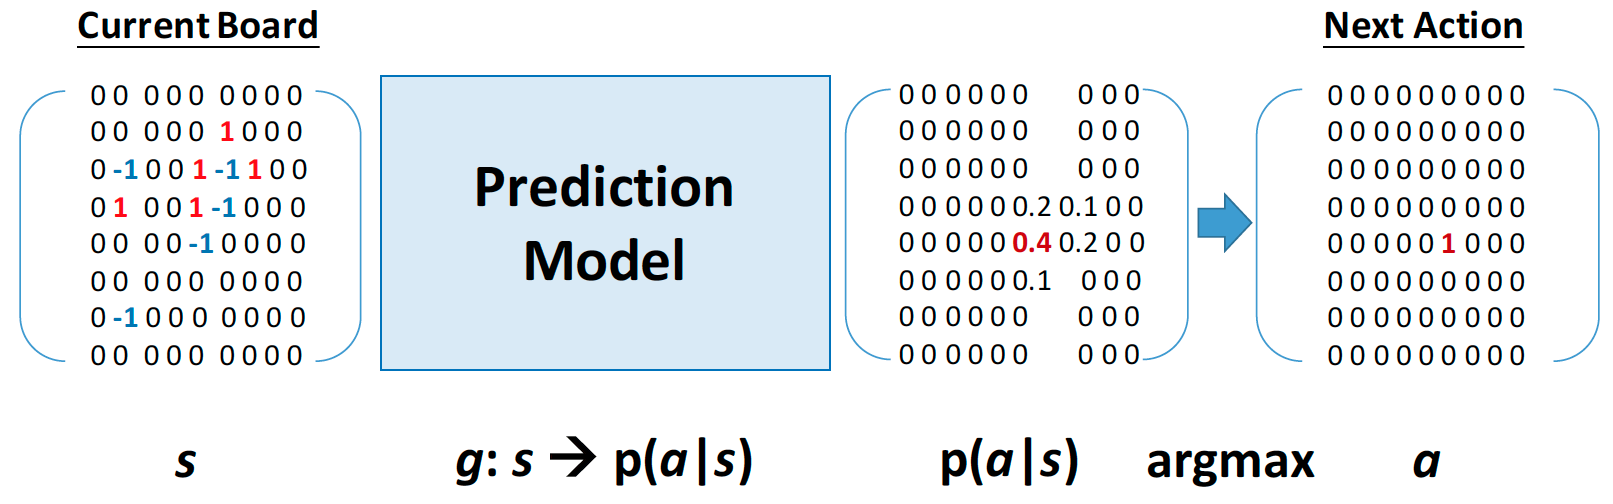
\includegraphics[width=0.9\textwidth]{figs/alphago4.png}
\end{figure}
\end{itemize}
\end{frame}

\begin{frame}
\frametitle{AlphaGo}
\begin{itemize}
\item Reducing ``action candidates'' (Breadth Reduction in Search Space)
\begin{itemize}
\item \tr{Policy Network}
\item Predicts the next action 
\end{itemize}
\item Board evaluation (Depth Reduction)
\begin{itemize}
\item \tr{Value Network}
\item Predicts values between 0 (a bad board position) to 1 (a good board position) 
\end{itemize}
\end{itemize}
\begin{figure}
      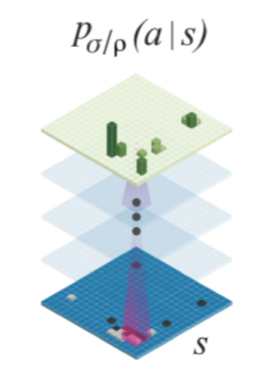
\includegraphics[width=0.23\textwidth]{figs/alphago6.png}
      \hspace{0.3in}
      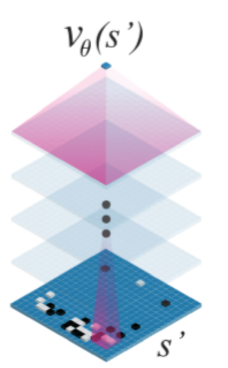
\includegraphics[width=0.21\textwidth]{figs/alphago7.png}
\end{figure}
\end{frame}

\begin{frame}
\frametitle{AlphaGo}
\begin{itemize}
\item Looking ahead: Monte Carlo Search Tree
\vspace{0.1in}
\begin{figure}
      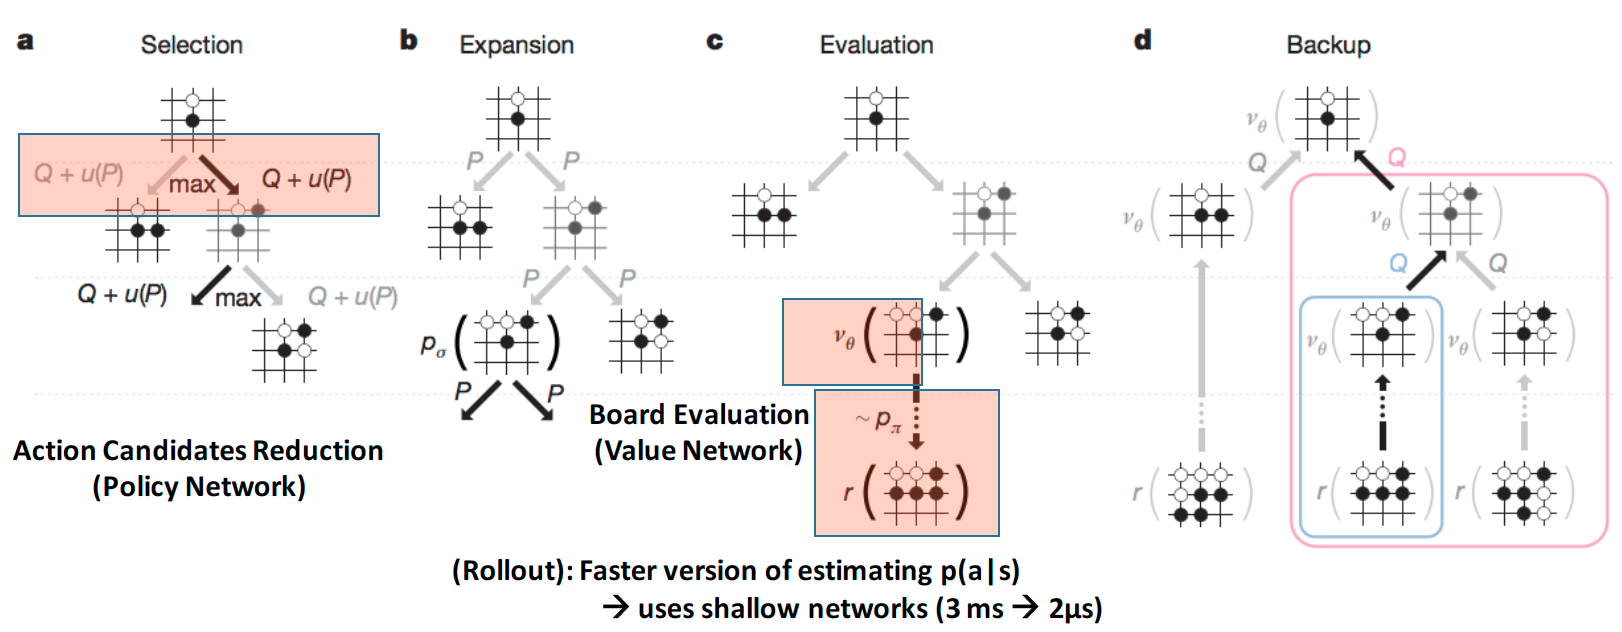
\includegraphics[width=0.93\textwidth]{figs/alphago8.png}
\end{figure}
\end{itemize}
\end{frame}

\begin{frame}
\frametitle{AlphaGo}
\begin{itemize}
\item Core problem: Learn $\mathbf{P(}$\textbf{next action}$ | $\textbf{current state}$\mathbf{)}$
\begin{figure}
      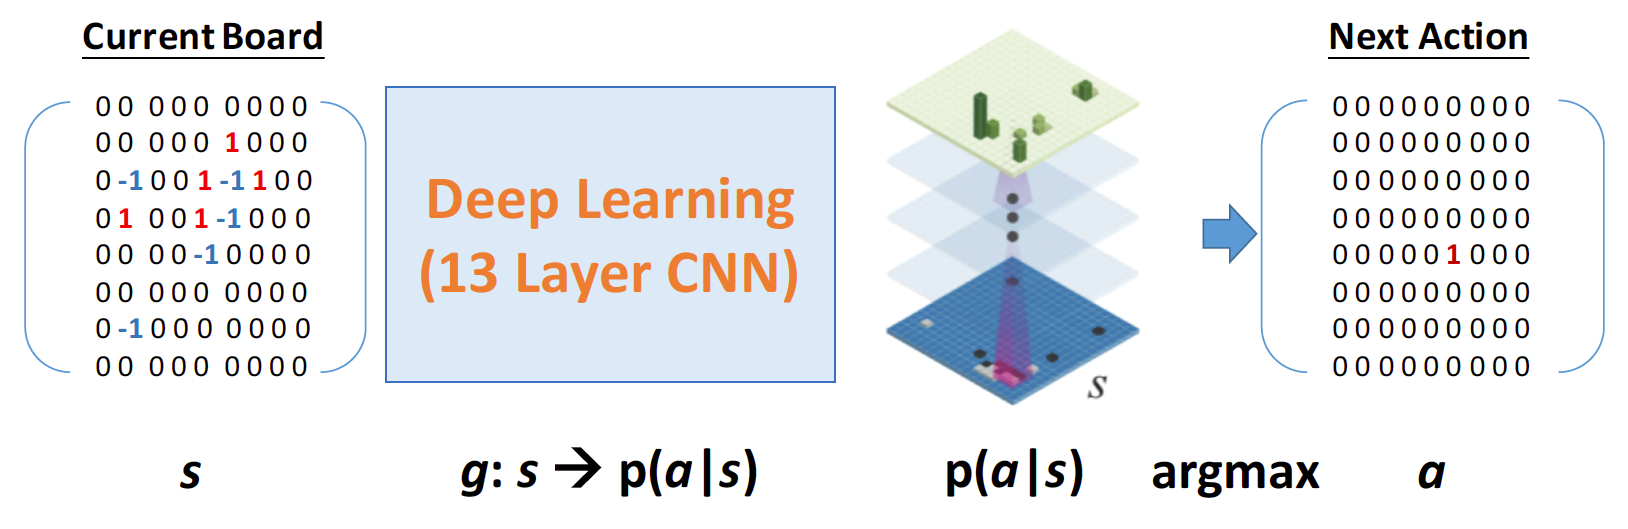
\includegraphics[width=0.9\textwidth]{figs/alphago5.png}
\end{figure}
\end{itemize}
\end{frame}

\begin{frame}
\frametitle{Large Scale Visual Recognition Challenge 2015}
\begin{itemize}
\item Scene classification: identify the scene category depicted in a photograph.
\item Data: \textbf{10+ million} images belonging to \textbf{400+} unique scene categories.
\item Champion: ResNet (MSRA)
\begin{itemize}
\item A very \textit{deep} network: depth of up to \tr{152} layers. 
\end{itemize}
\begin{figure}
      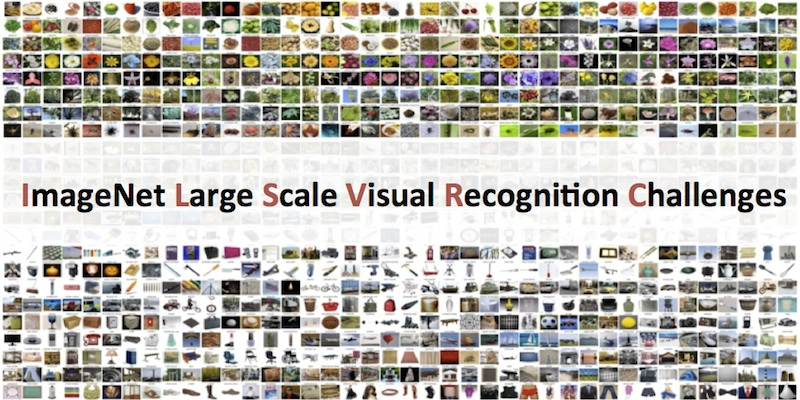
\includegraphics[width=0.75\textwidth]{figs/ca-ilsvrc.jpg}
\end{figure}
\end{itemize}
\end{frame}

\begin{frame}
\frametitle{Example of ResNet (Right: 34 parameter layers ResNet)}
\begin{figure}
      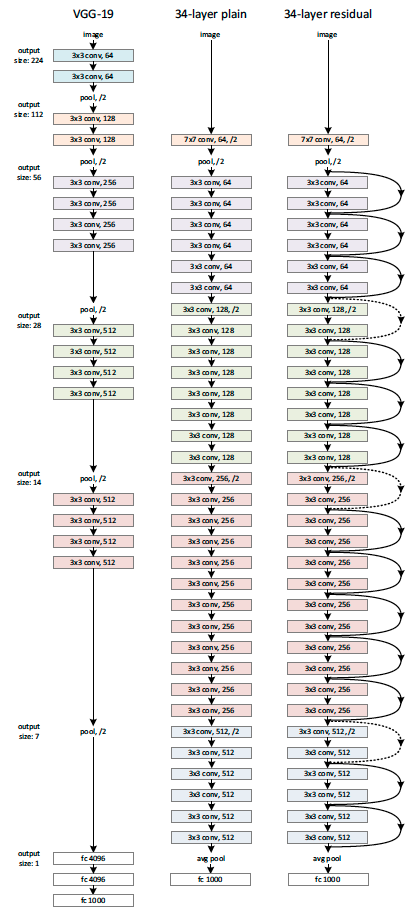
\includegraphics[width=0.3\textwidth]{figs/resnet.png}
\end{figure}
\end{frame}

\begin{frame}
\frametitle{Deep Learning = Learning Representations/Features}
\begin{figure}
      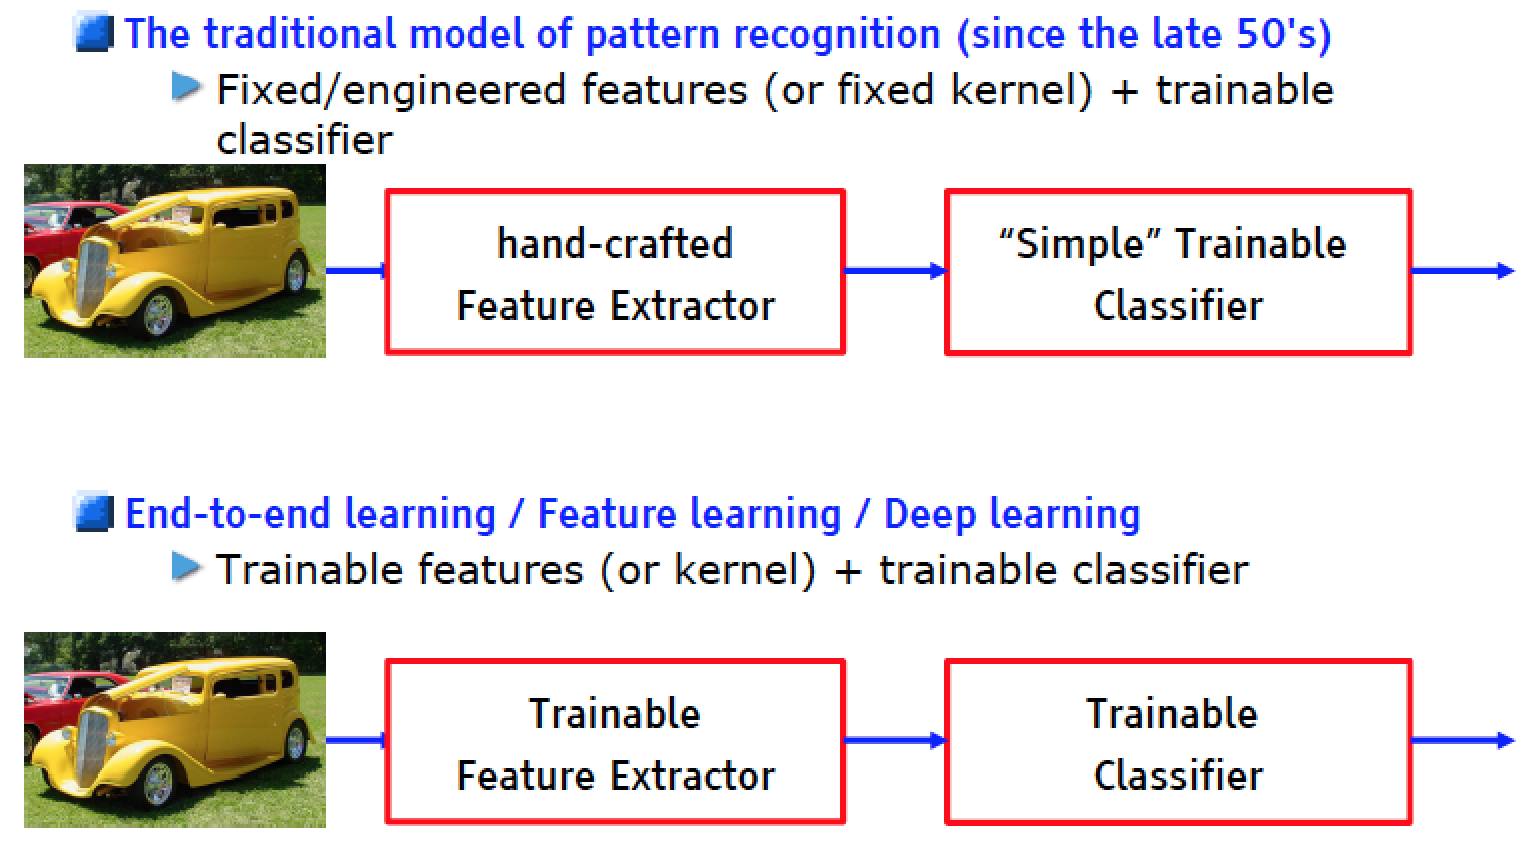
\includegraphics[width=1\textwidth]{figs/intro1.png}
\end{figure}
\end{frame}

\begin{frame}
\frametitle{Architecture of Mainstream Pattern Recognition Systems}
\begin{figure}
      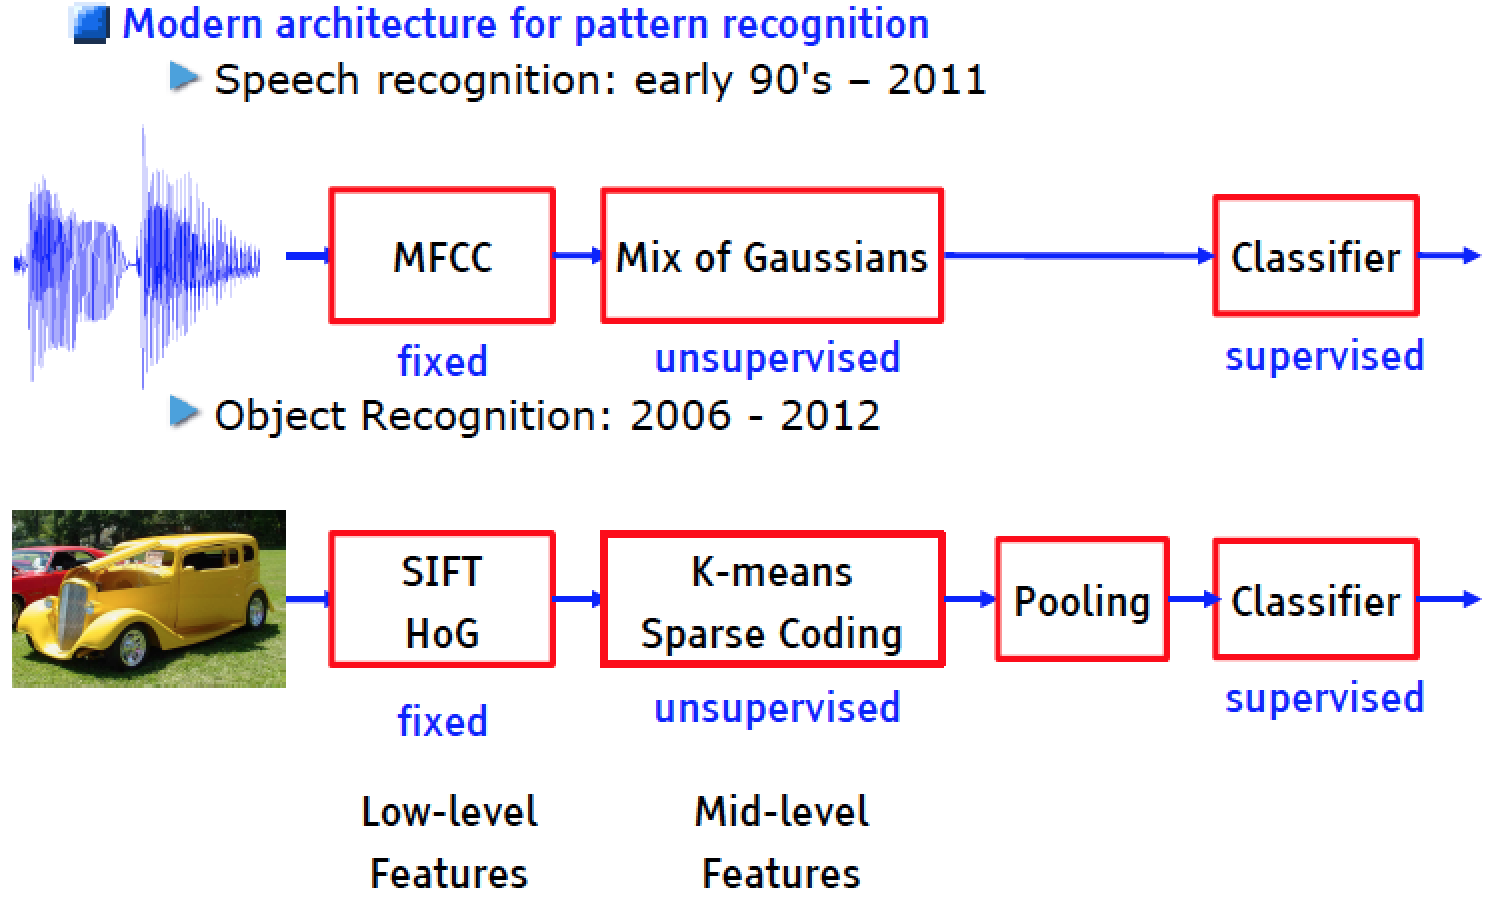
\includegraphics[width=1\textwidth]{figs/intro2.png}
\end{figure}
\end{frame}

\begin{frame}
\frametitle{Deep Learning = Learning Hierarchical Representations}
\begin{figure}
      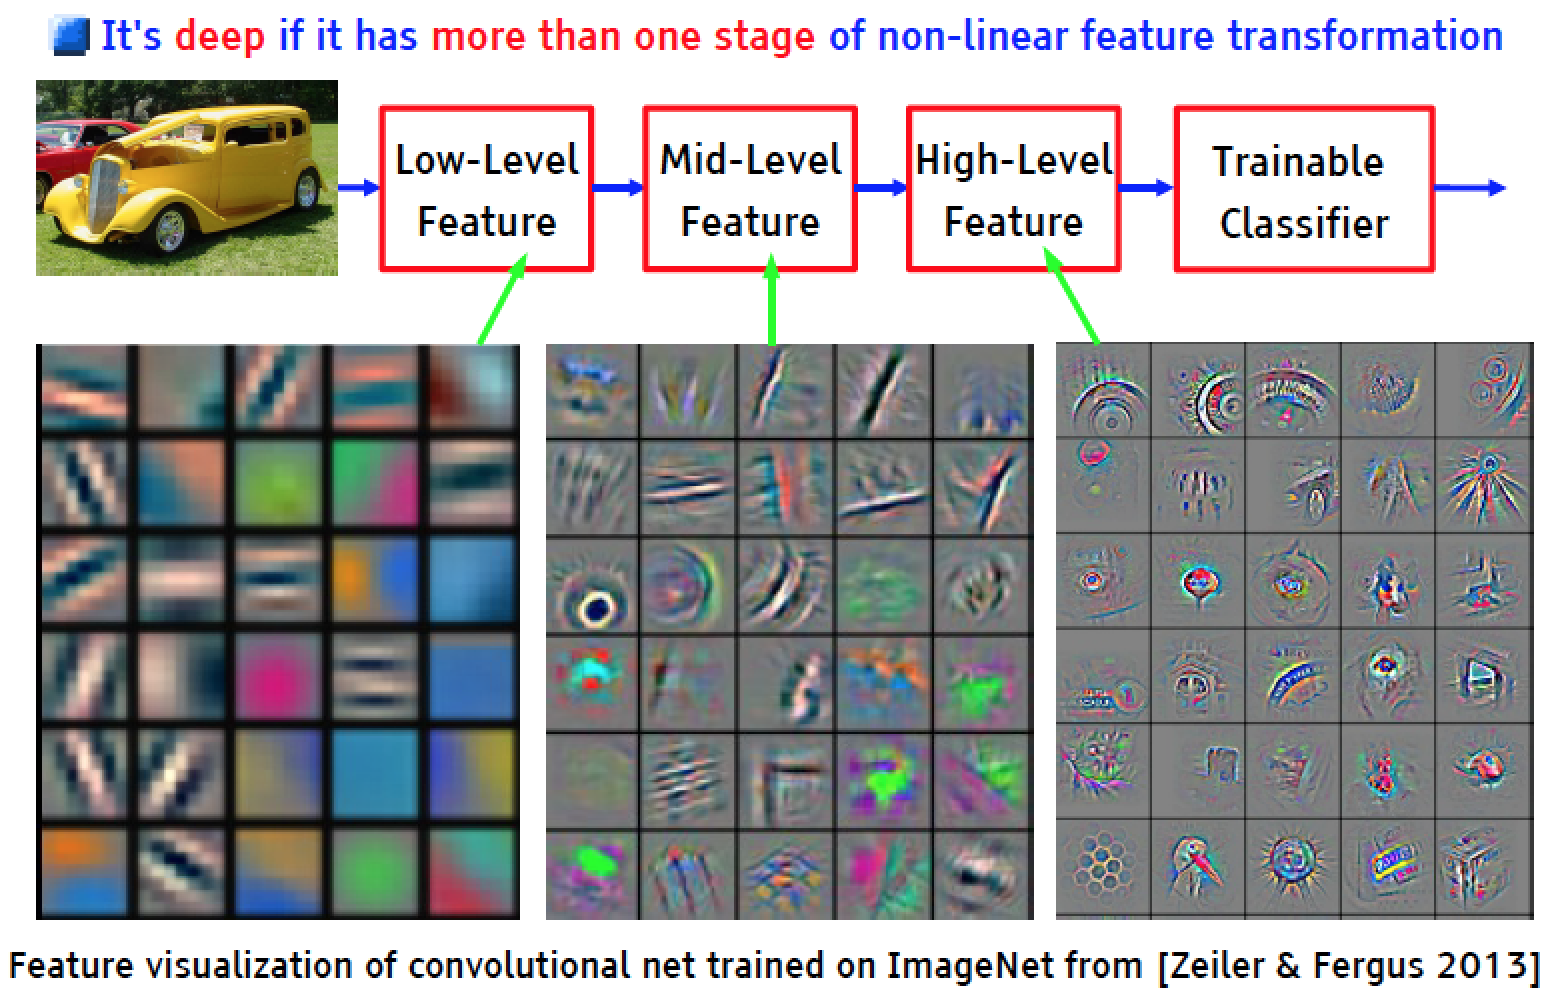
\includegraphics[width=1\textwidth]{figs/intro3.png}
\end{figure}
\end{frame}

\begin{frame}
\frametitle{Trainable Feature Hierarchy}
\begin{figure}
      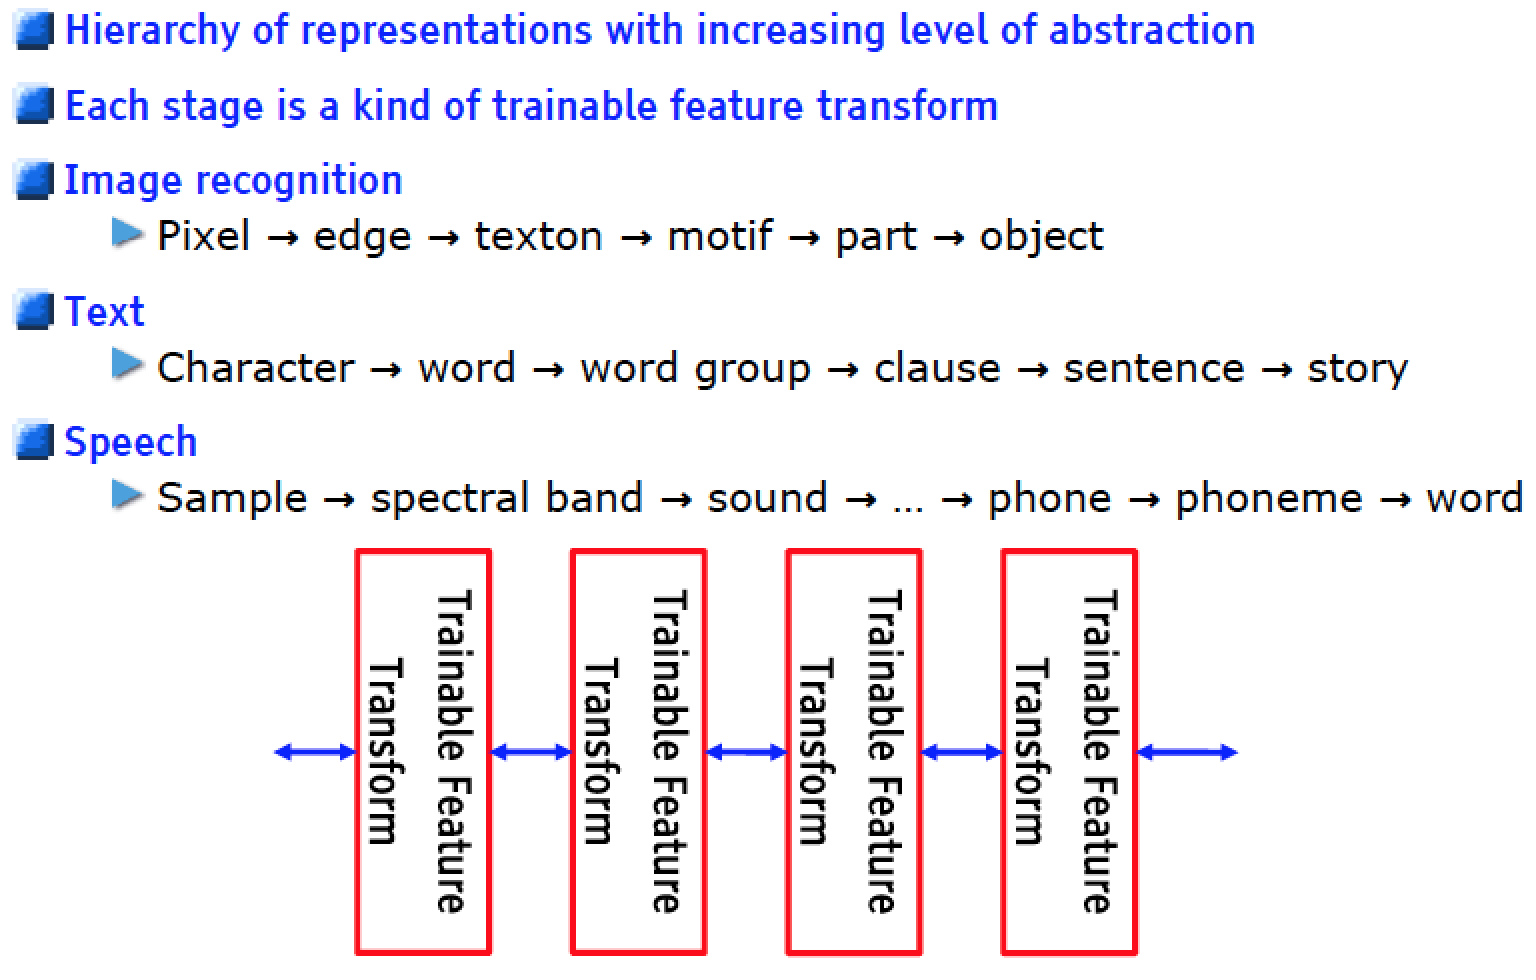
\includegraphics[width=1\textwidth]{figs/intro4.png}
\end{figure}
\end{frame}

\begin{frame}
\frametitle{The Mammalian Visual Cortex is Hierarchical}
\begin{figure}
      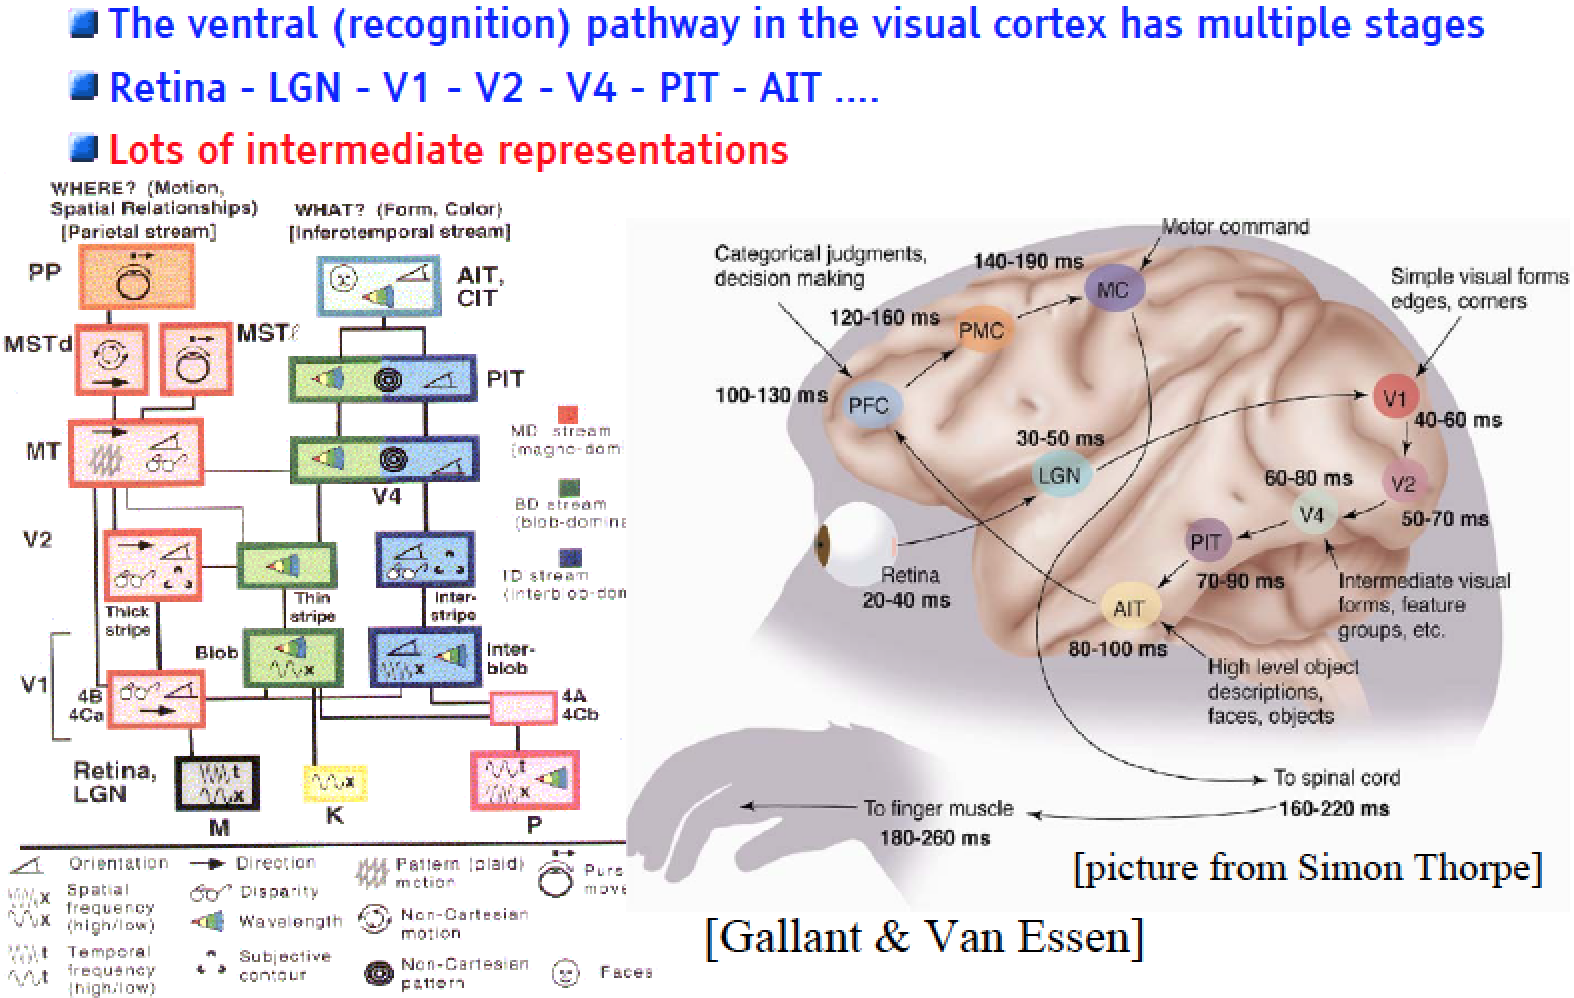
\includegraphics[width=1\textwidth]{figs/intro5.png}
\end{figure}
\end{frame}

\hide{
\begin{frame}
\frametitle{Inspired By Nature, But Not Too Much}
\begin{figure}
      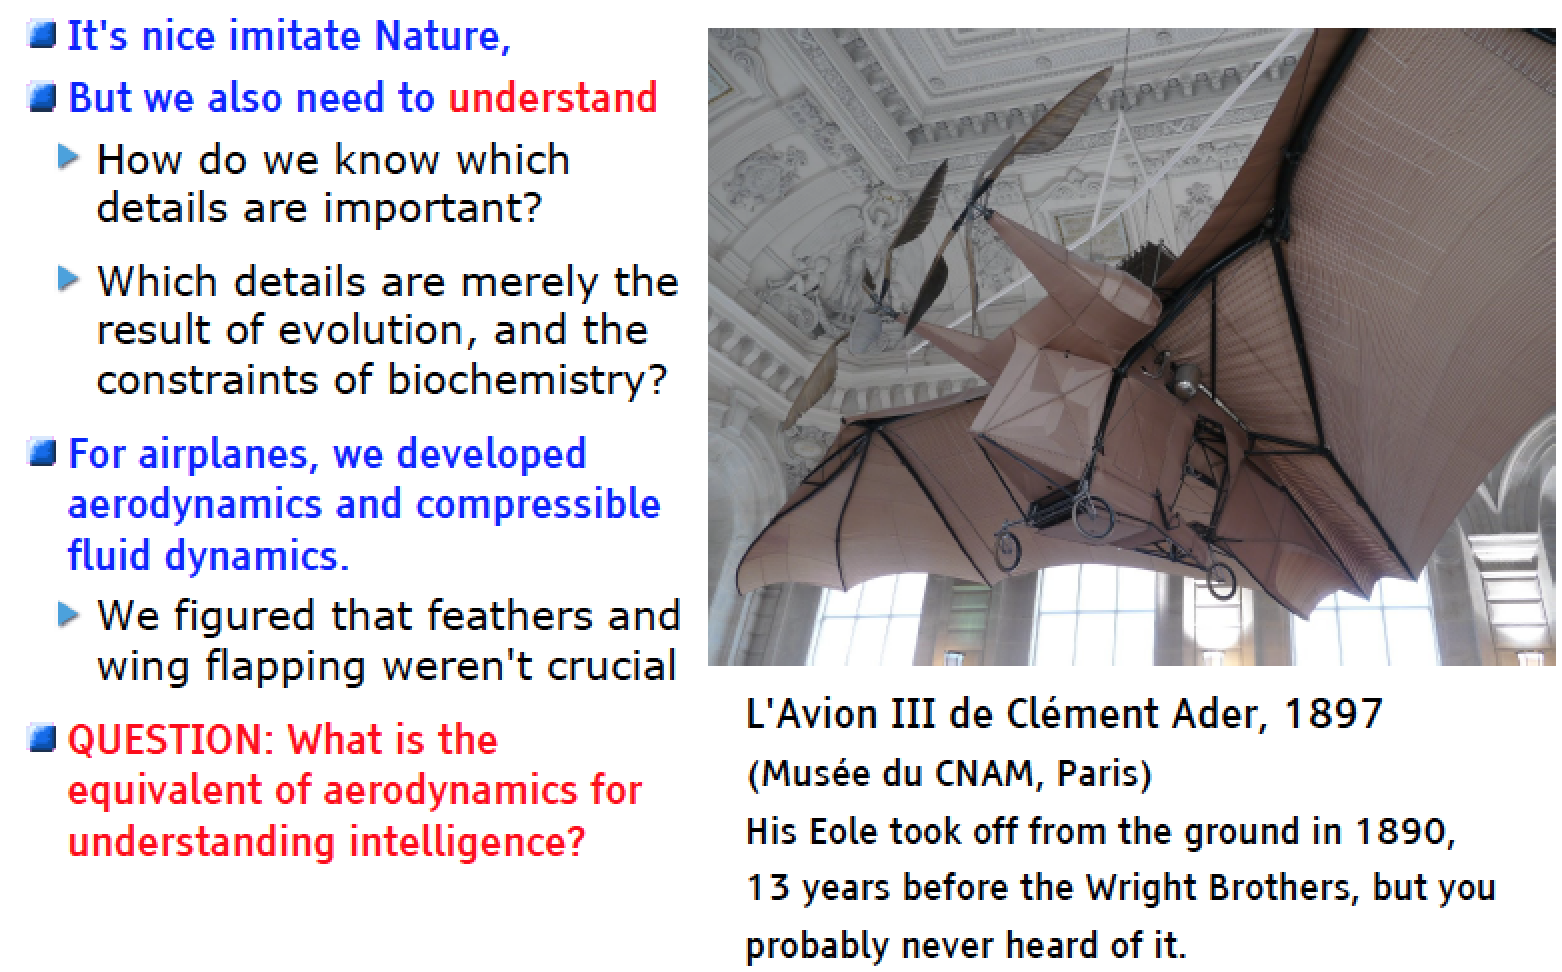
\includegraphics[width=1\textwidth]{figs/intro6.png}
\end{figure}
\end{frame}
}

\begin{frame}
\frametitle{Three Types of Deep Architectures}
\begin{figure}
      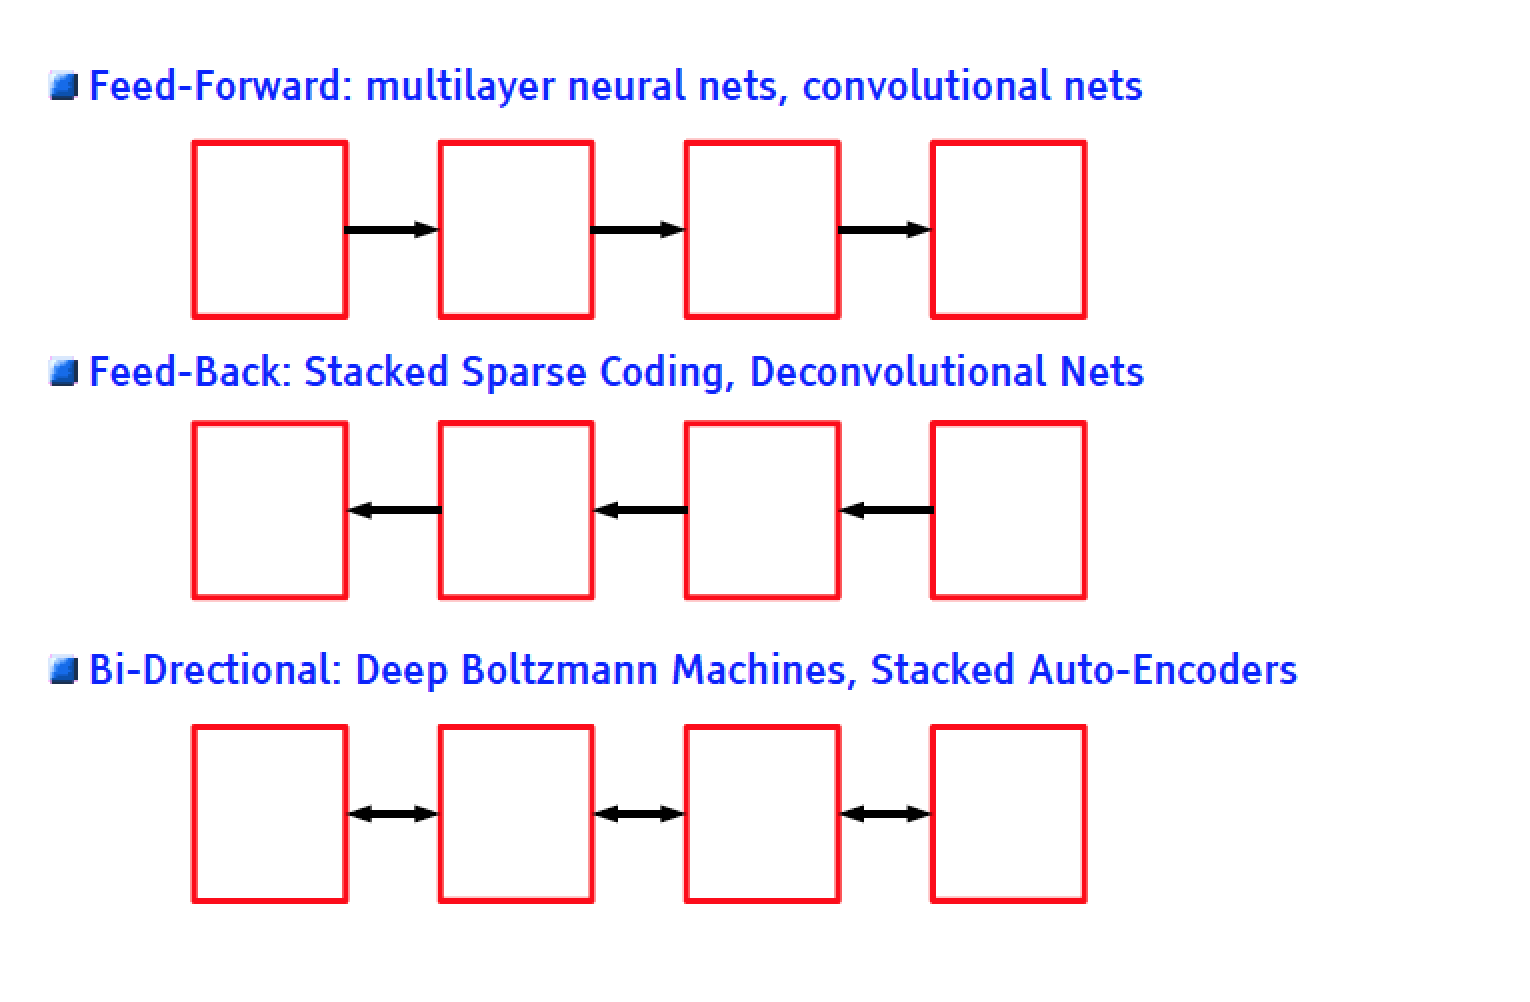
\includegraphics[width=1\textwidth]{figs/intro7.png}
\end{figure}
\end{frame}

\begin{frame}
\frametitle{Three Types of Training Protocols}
\begin{figure}
      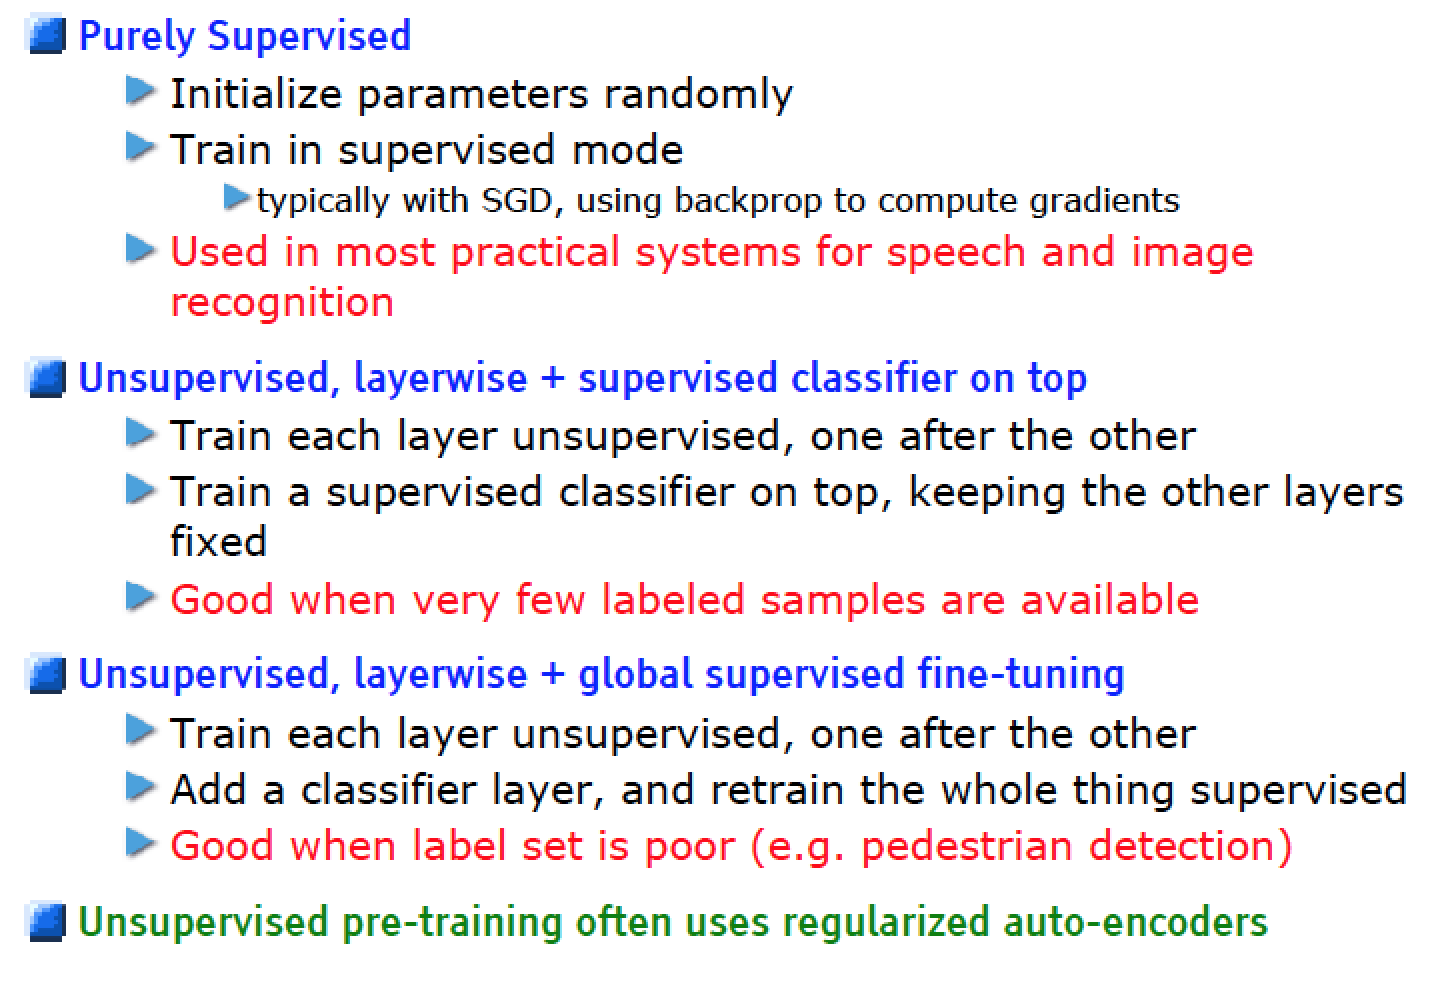
\includegraphics[width=1\textwidth]{figs/intro8.png}
\end{figure}
\end{frame}

\begin{frame}
\frametitle{Which Models are Deep?}
\begin{figure}
      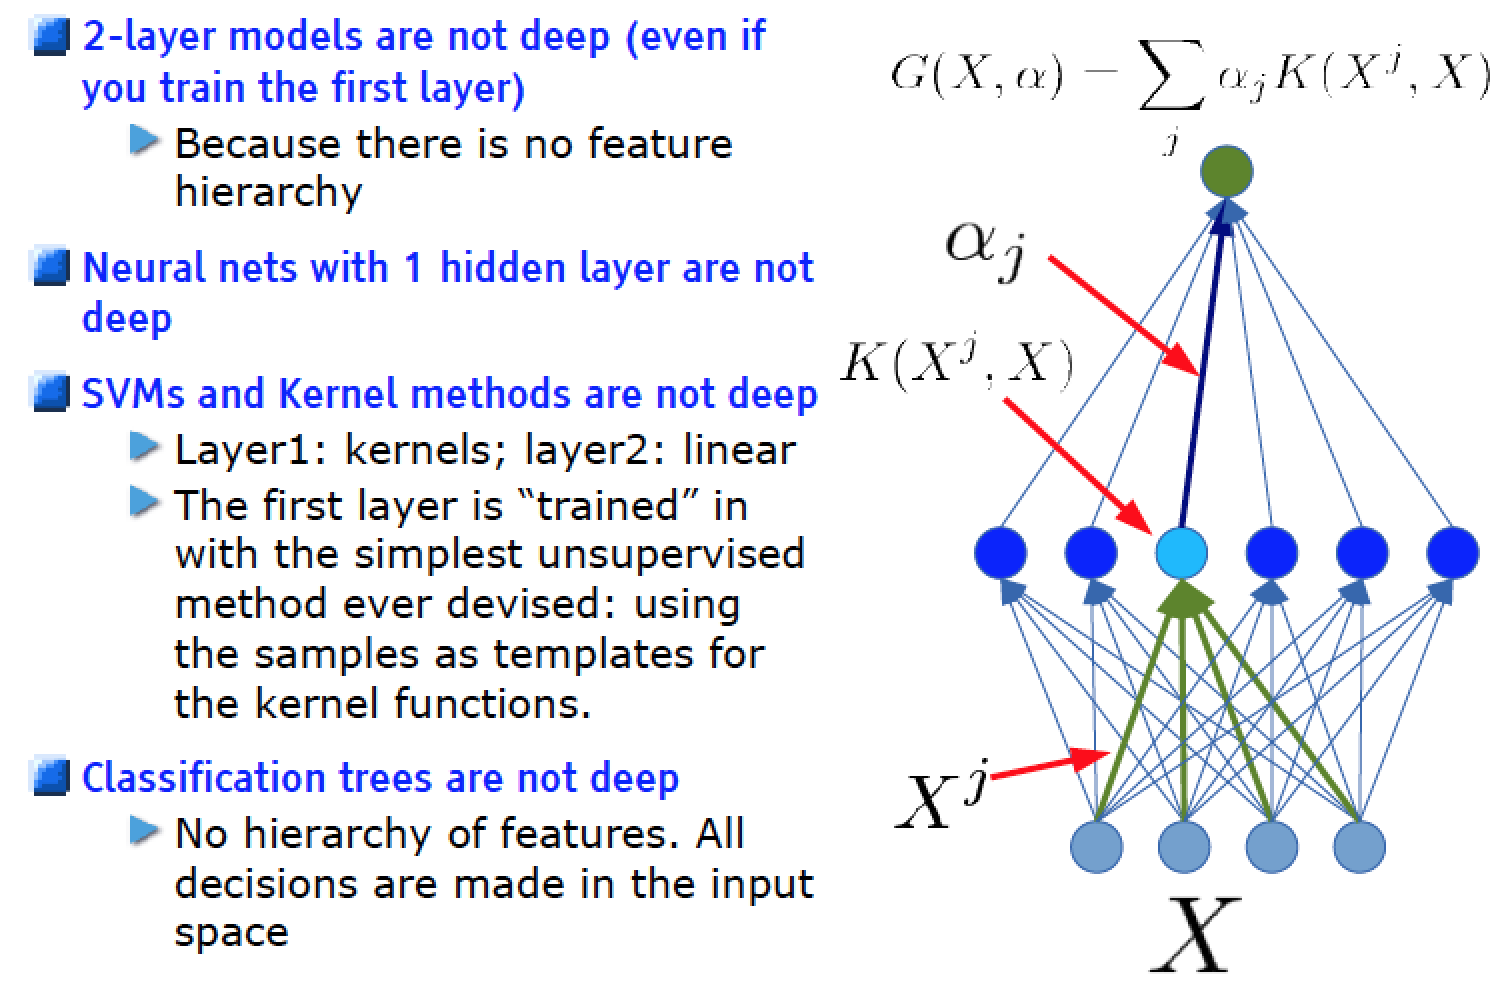
\includegraphics[width=1\textwidth]{figs/intro9.png}
\end{figure}
\end{frame}

\begin{frame}
\frametitle{Are Graphical Models Deep?}
\begin{figure}
      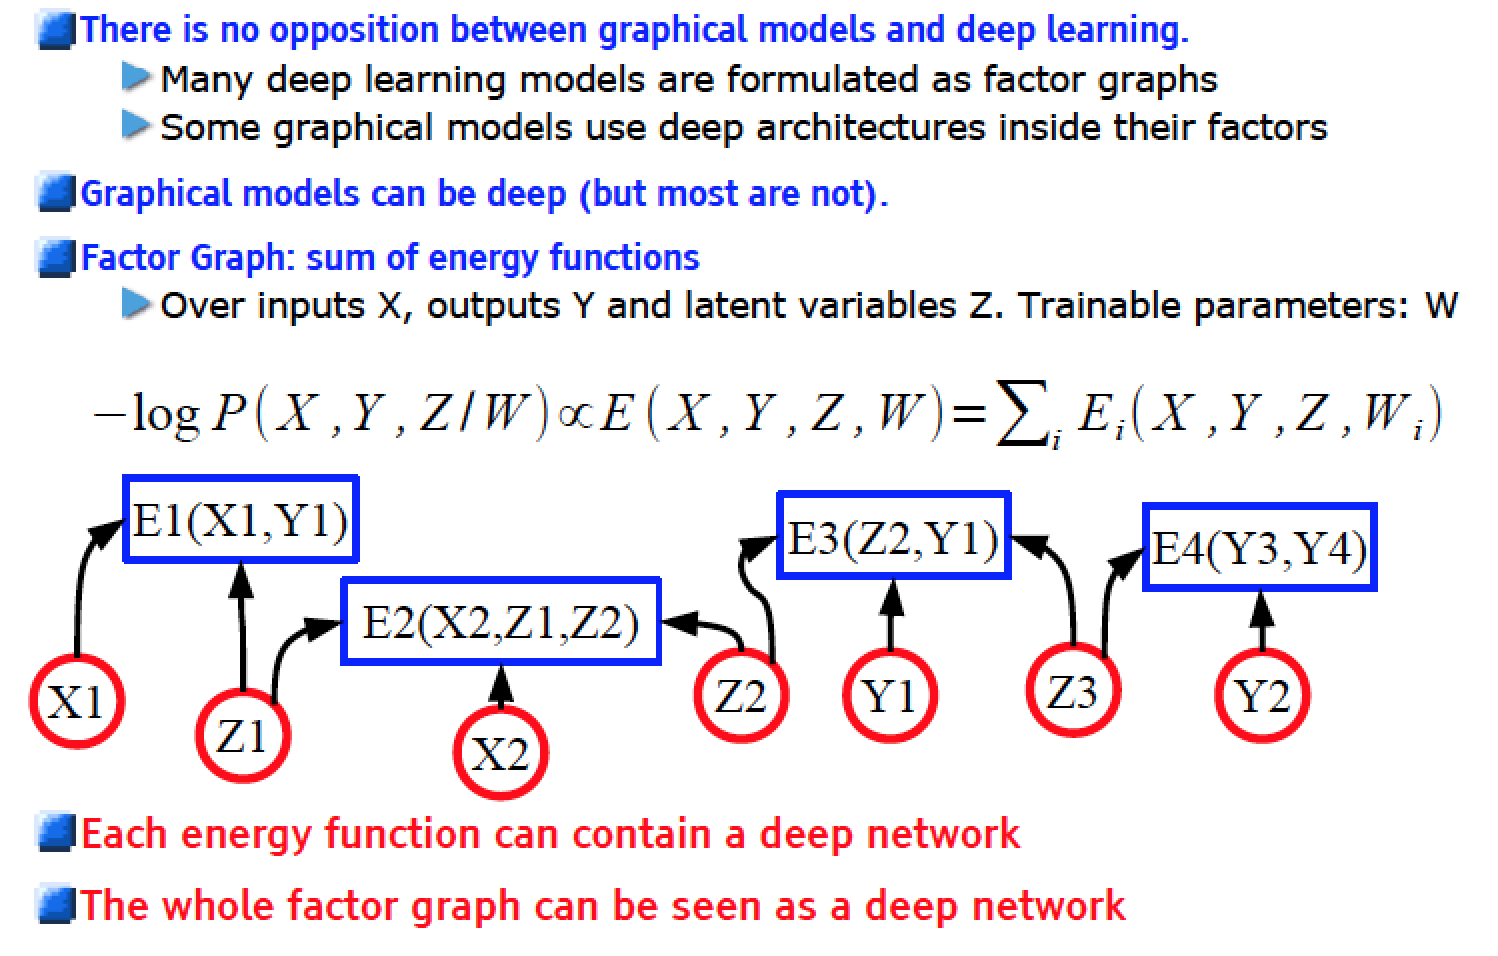
\includegraphics[width=1\textwidth]{figs/intro10.png}
\end{figure}
\end{frame}

\begin{frame}
\frametitle{Deep Learning: A Theoretician's Nightmare?}
\begin{figure}
      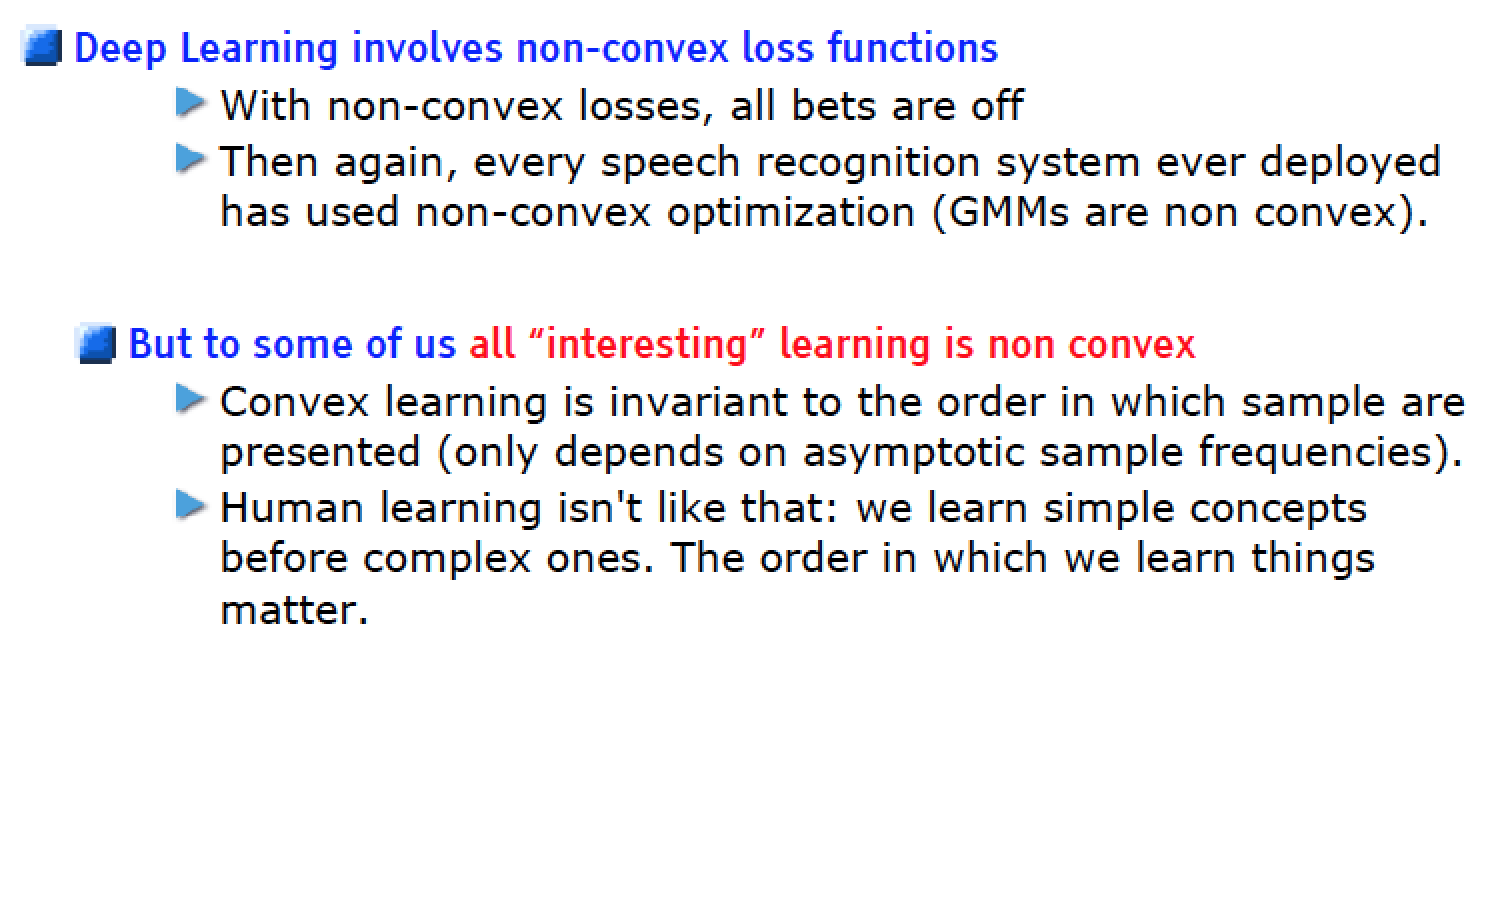
\includegraphics[width=1\textwidth]{figs/intro11.png}
\end{figure}
\end{frame}

\begin{frame}
\frametitle{Deep Learning: A Theoretician's Nightmare?}
\begin{figure}
      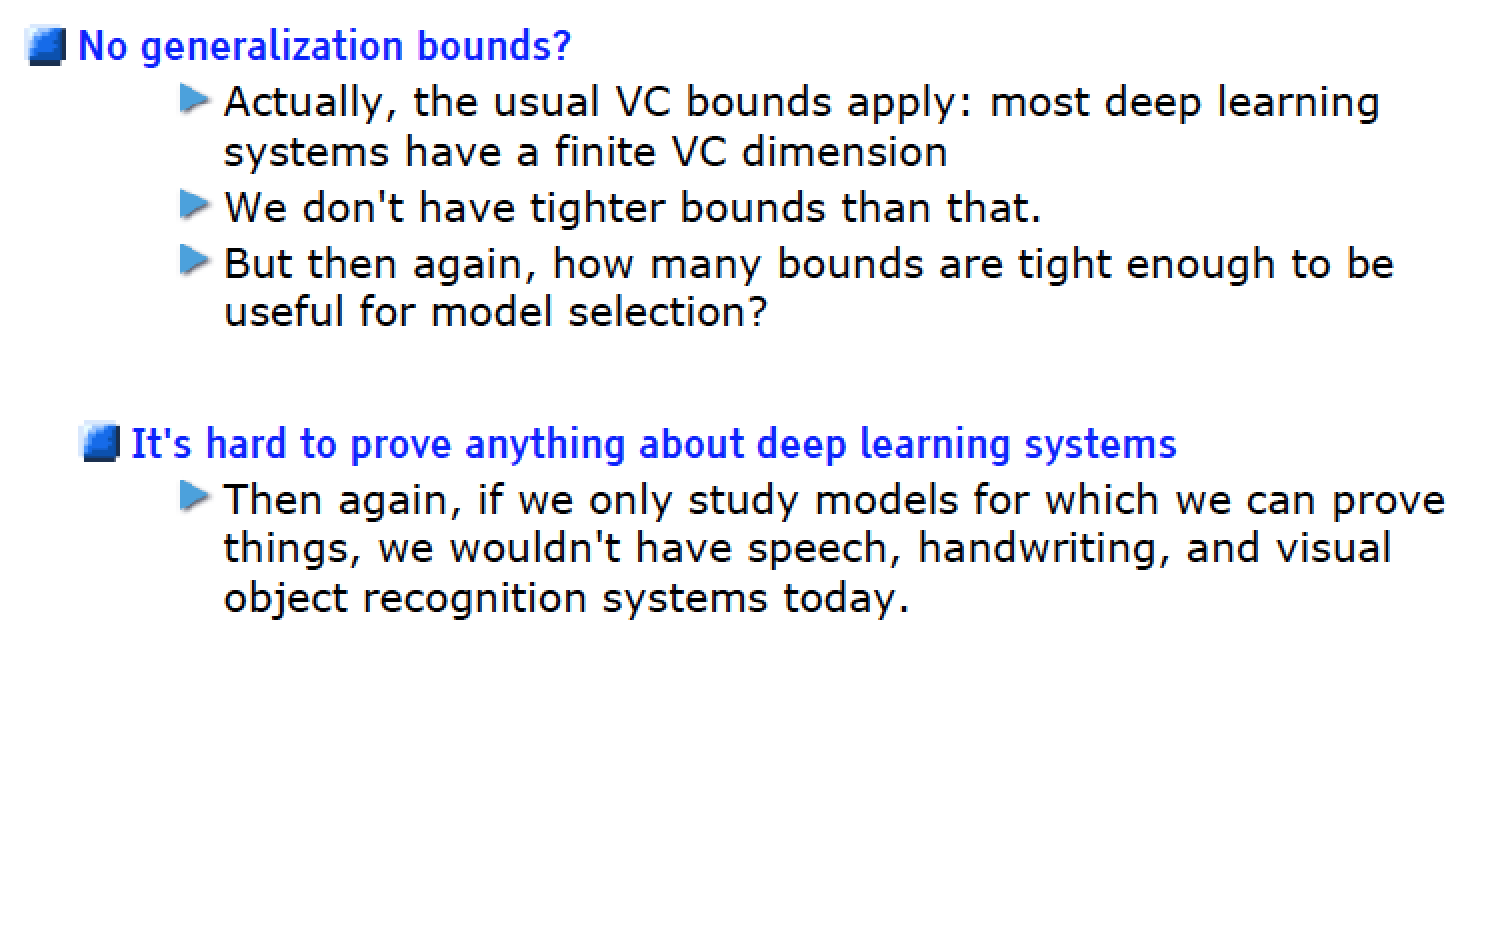
\includegraphics[width=1\textwidth]{figs/intro12.png}
\end{figure}
\end{frame}

\hide{
\begin{frame}
\frametitle{Discovering Hidden Structure in High-Dimensional Data}
\begin{figure}
      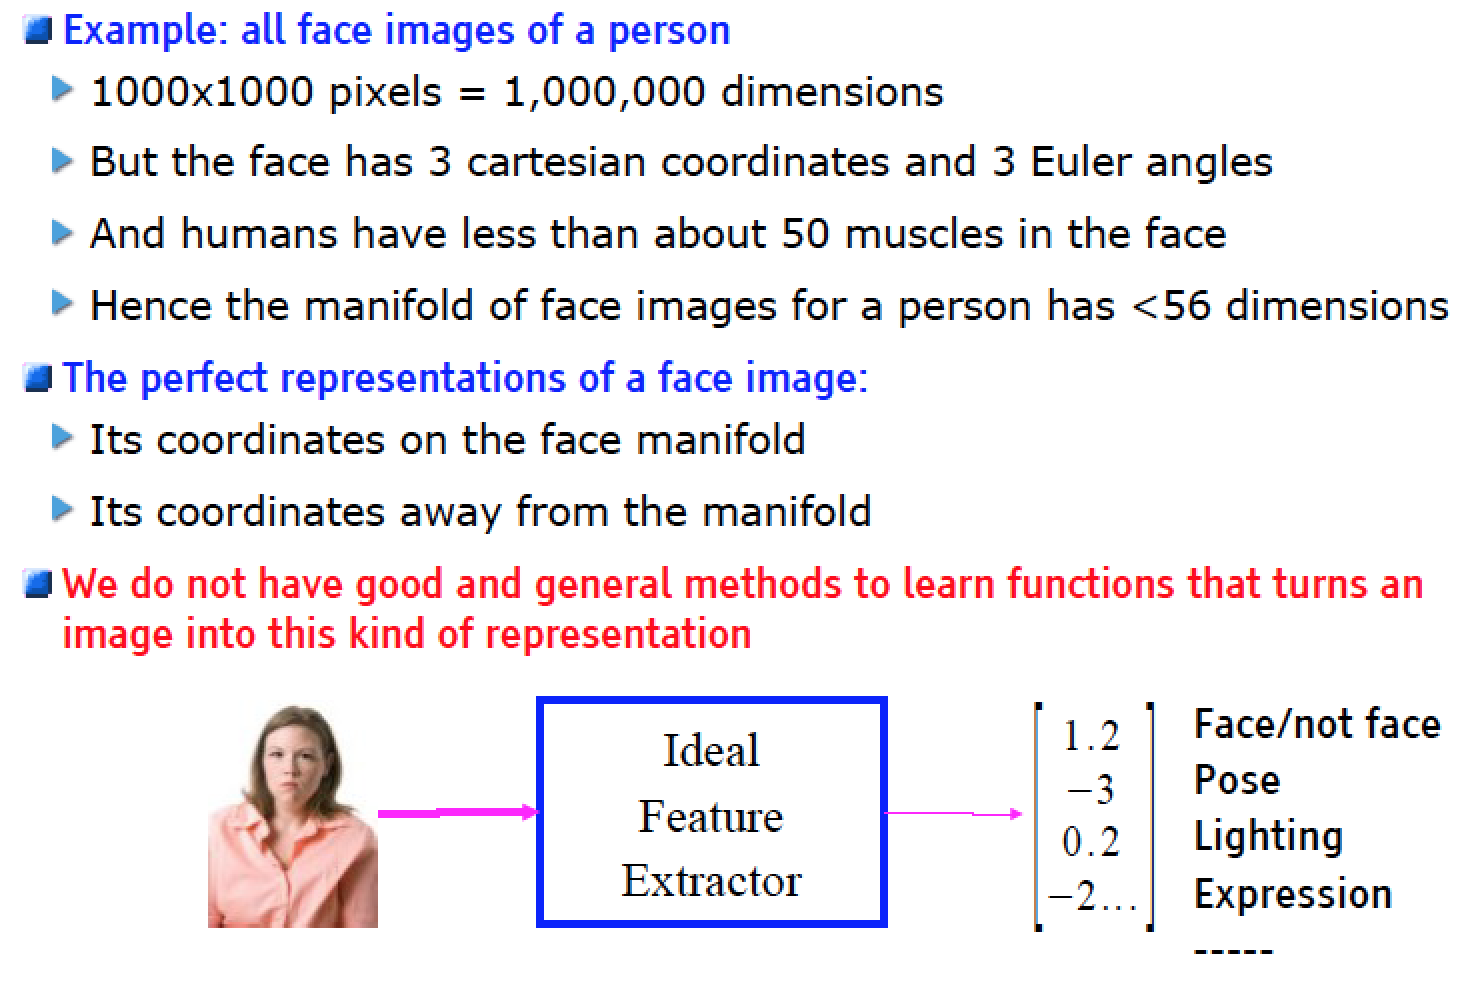
\includegraphics[width=1\textwidth]{figs/intro13.png}
\end{figure}
\end{frame}

\begin{frame}
\frametitle{Disentangling Factors of Variation}
\begin{figure}
      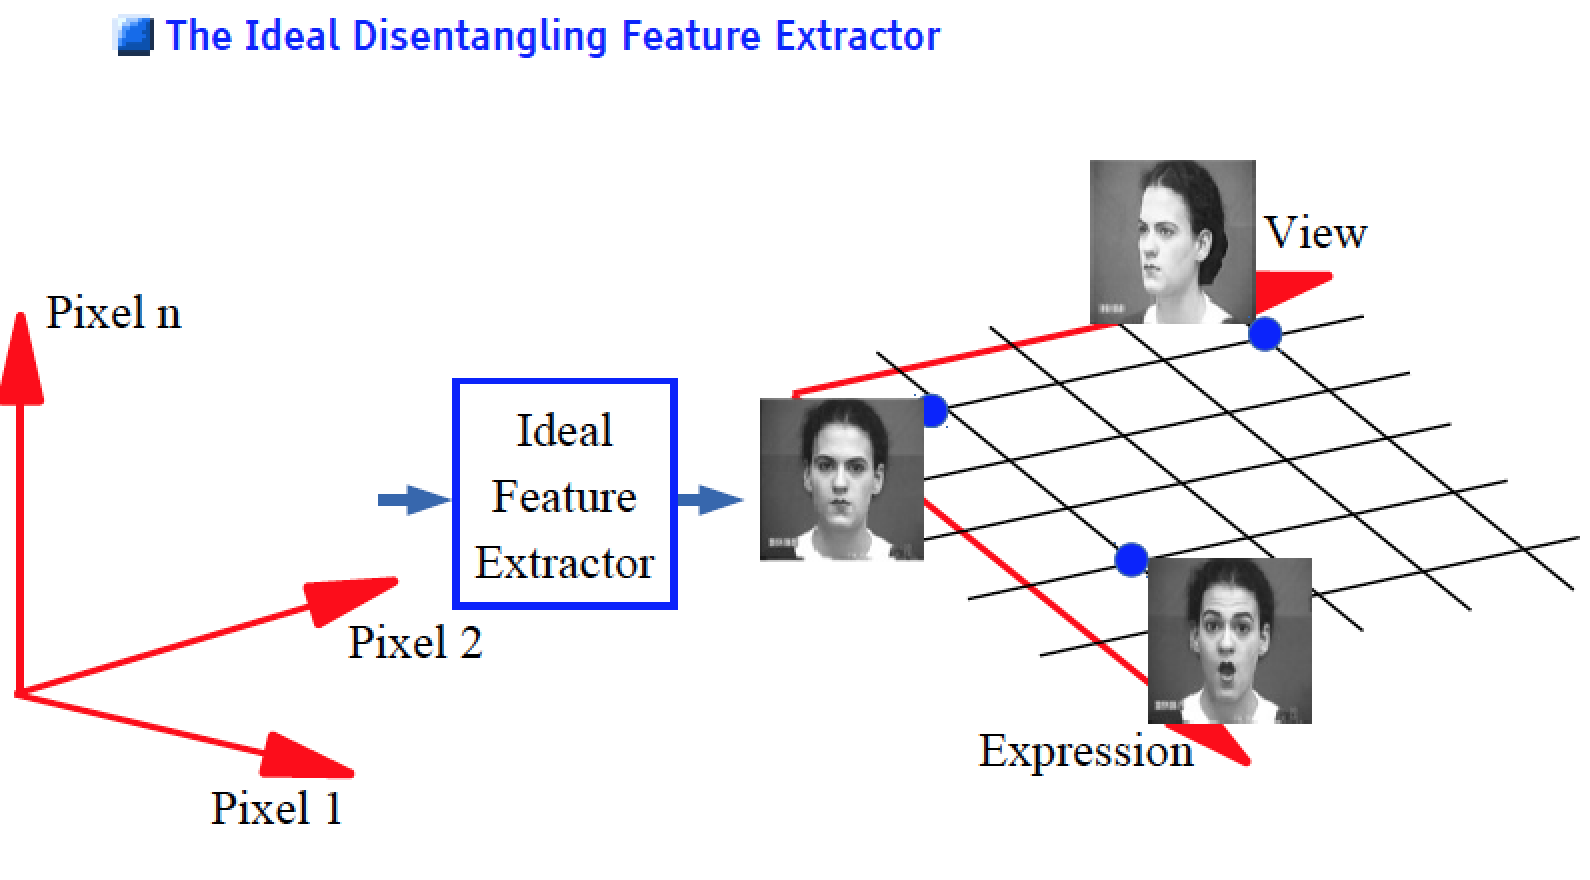
\includegraphics[width=1\textwidth]{figs/intro14.png}
\end{figure}
\end{frame}

\begin{frame}
\frametitle{Overall Architecture}
\begin{figure}
      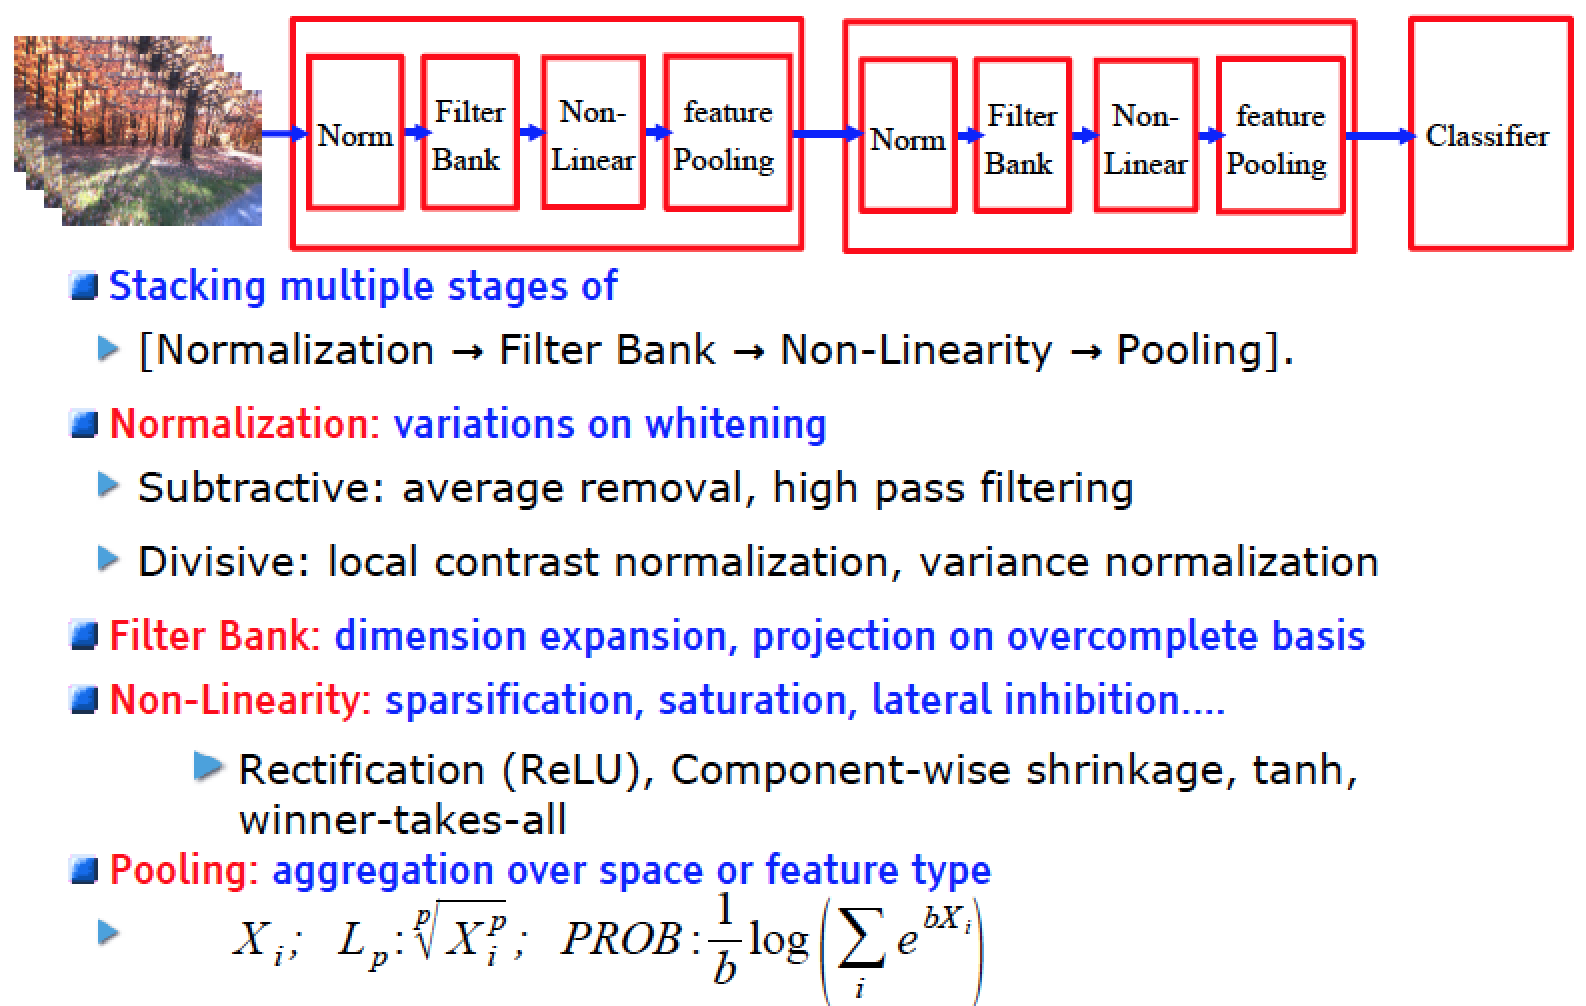
\includegraphics[width=1\textwidth]{figs/intro15.png}
\end{figure}
\end{frame}
}

\section{Neural Network}

\begin{frame}
  \frametitle{Contents}
  \tableofcontents[currentsection]
\end{frame}

\begin{frame}
\frametitle{Neural Network}
\begin{itemize}
\item Consider a supervised learning problem where we have access to labeled training examples $(x^{(i)}, y^{(i)})$.
\item Neural networks give a way of defining a complex, non-linear form of hypotheses $h_{W,b}(x)$, with parameters $W, b$ that we can fit to our data.
\item To describe neural networks, we will begin by describing the simplest possible neural network, one which comprises a single \tr{``neuron''}. 

\begin{figure}
      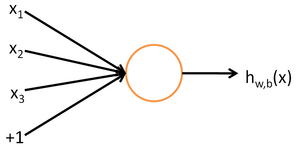
\includegraphics[height=2.6cm]{figs/SingleNeuron.png}
\end{figure}

%\item $h_{W,b}(x)=f(W^{T}x)=f(\sum_{i=1}^{3}W_ix_i+b)$, where $f: \mathcal{R} \rightarrow \mathcal{R}$ is called the activation function.

\end{itemize}
\end{frame}

\begin{frame}
\frametitle{Activation Function}

\begin{figure}
      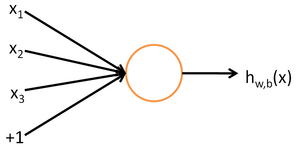
\includegraphics[height=2.6cm]{figs/SingleNeuron.png}
\end{figure}

\begin{itemize}
\item $h_{W,b}(x)=f(W^{T}x)=f(\sum_{i=1}^{3}W_ix_i+b)$, where $f: \mathcal{R} \rightarrow \mathcal{R}$ is called the \tr{activation function}.
\item Normally, we choose $f(\cdot)$ to be the \tb{sigmoid function}:
\beq{
f(z)=\frac{1}{1+e^{-z}}
}
\item Another common choice for $f$ is the \tb{hyperbolic tangent}, or \tb{tanh}, function:
\beq{
f(z)=tanh(z)=\frac{e^{z}-e^{-z}}{e^{z}+e^{-z}}
}
\end{itemize}

\end{frame}

\begin{frame}
\frametitle{Activation Function}
\begin{itemize}
\item Plots of the sigmoid and tanh functions:
\begin{figure}
      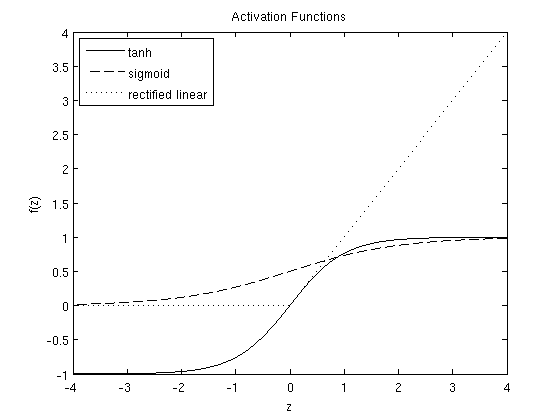
\includegraphics[height=4cm]{figs/Activation_functions.png}
\end{figure}

\item The $tanh(z)$ function is a rescaled version of the sigmoid, and its output range is $[-1,1]$ instead of $[0,1]$. 

\end{itemize}
\end{frame}

\begin{frame}
\frametitle{Neural Network Model}
\begin{itemize}
\item A neural network is put together by hooking together many of our simple "neurons," so that the output of a neuron can be the input of another. 
\begin{figure}
      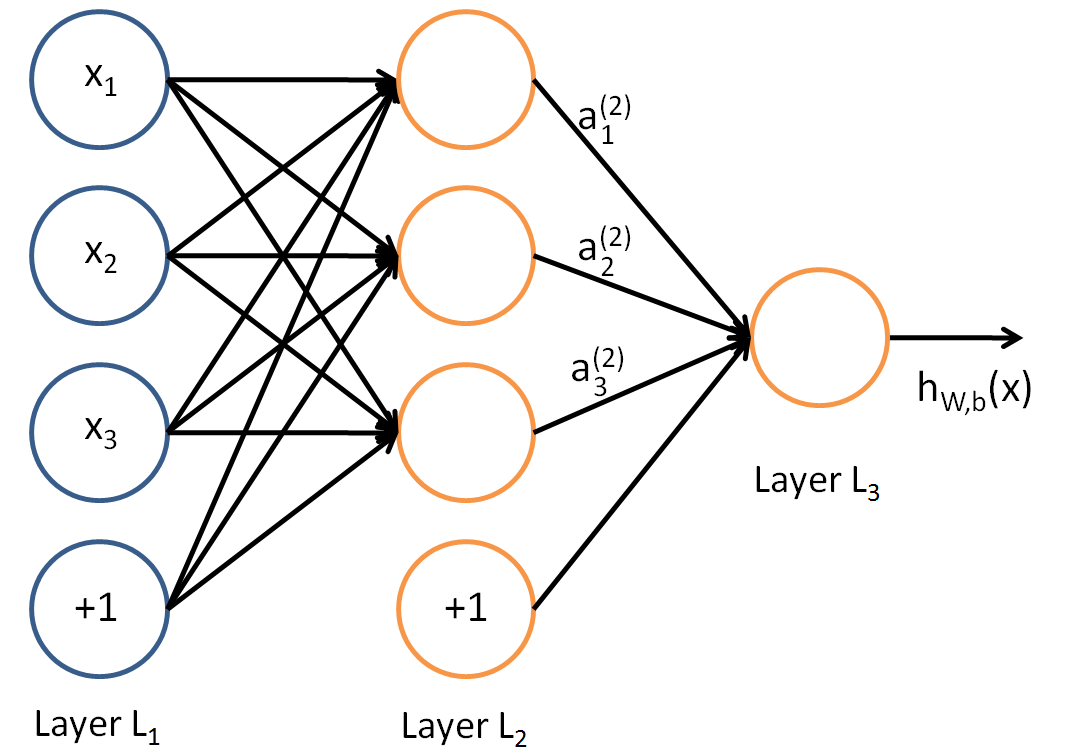
\includegraphics[height=3cm]{figs/Network331.png}
\end{figure}

\item The leftmost layer of the network is called the \textbf{input layer}, and the rightmost layer the \textbf{output layer}.
\item The middle layer of nodes is called the \textbf{hidden layer}, because its values are not observed in the training set. 
\item The circles labeled ``+1'' are called \textbf{bias units}, and correspond to the intercept term (don't have inputs or connections going into them, since they always output the value +1).
\end{itemize}
\end{frame}

\begin{frame}
\frametitle{Model Computation}
\begin{itemize}
\item Let $W_{ij}^{(l)}$ denote the parameter (or weight) associated with the connection between unit $j$ in layer $l$, and unit $i$ in layer $l + 1$.
\item Let $b_i^{(l)}$ denote the bias associated with unit $i$ in layer $l + 1$. 
\item Let $a_i^{(l)}$ to denote the \textbf{activation} (meaning output value) of unit $i$ in layer $l$. For $l=1$, we also use $a_i^{(1)}=x_i$ to the i-th input.
\item Given a fixed setting of the parameters $W,b$, the neural network defines a hypothesis $h_{W,b}(x)$ that outputs a real number. 
\hide{
\beqn{
a_1^{(2)} &=& f(W_{11}^{(1)}x_1+W_{12}^{(1)}x_+W_{13}^{(1)}x_3+b_1^{(1)})\\
a_2^{(2)} &=& f(W_{21}^{(1)}x_1+W_{22}^{(1)}x_+W_{23}^{(1)}x_3+b_1^{(1)})\\
a_3^{(2)} &=& f(W_{31}^{(1)}x_1+W_{32}^{(1)}x_+W_{33}^{(1)}x_3+b_1^{(1)})\\
h_{W,b}(x) &=& a_1^{(3)}=f(W_{11}^{(2)}a_1^{(2)}+W_{12}^{(2)}a_2^{(2)}+W_{13}^{(2)}a_3^{(2)}+b_1^{(2)})
}
}
\end{itemize}
\end{frame}

\begin{frame}
\frametitle{Model Computation}
\begin{figure}
      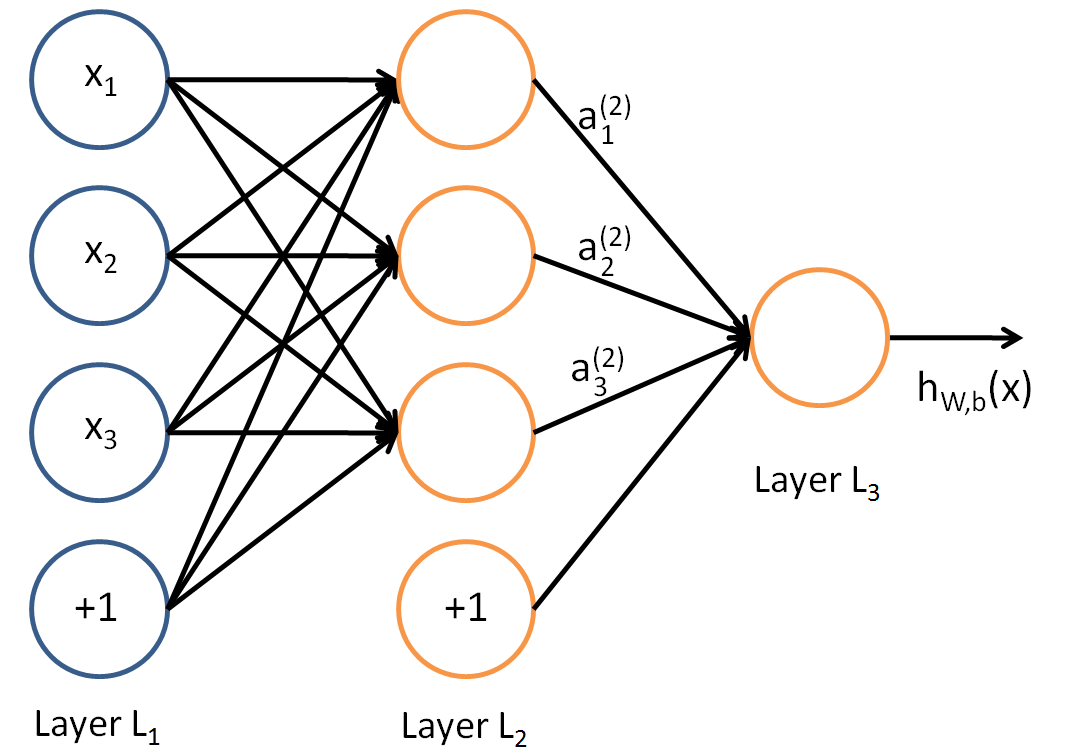
\includegraphics[height=3cm]{figs/Network331.png}
\end{figure}
\beqn{
a_1^{(2)} &=& f(W_{11}^{(1)}x_1+W_{12}^{(1)}x_2+W_{13}^{(1)}x_3+b_1^{(1)})\\
a_2^{(2)} &=& f(W_{21}^{(1)}x_1+W_{22}^{(1)}x_2+W_{23}^{(1)}x_3+b_1^{(1)})\\
a_3^{(2)} &=& f(W_{31}^{(1)}x_1+W_{32}^{(1)}x_2+W_{33}^{(1)}x_3+b_1^{(1)})\\
h_{W,b}(x) &=& a_1^{(3)}=f(W_{11}^{(2)}a_1^{(2)}+W_{12}^{(2)}a_2^{(2)}+W_{13}^{(2)}a_3^{(2)}+b_1^{(2)})
}
\end{frame}

\begin{frame}
\frametitle{Forward Propagation}
\begin{itemize}
\item More generally:
\beqn{
z^{(l+1)}&=& W^{(l)}a^{(l)}+b^{(l)} \\
a^{(l+1)}&=& f(z^{(l+1)})
}
\item We call this activation computation process as \textbf{forward propagation}.
\end{itemize}
\end{frame}

\begin{frame}
\frametitle{Model Building}
\begin{itemize}
\item We can build neural networks with other \textbf{architectures} (meaning patterns of connectivity between neurons), including ones with multiple hidden layers.
\item The most common choice is a $n_l$-layered network where layer $1$ is the input layer, layer $n_l$ is the output layer, and each layer $l$ is densely connected to layer $l+1$.
\item In this setting, to compute the output of the network, we can successively compute all the activations in layer $L_2$, then layer $L_3$, and so on, up to layer $L_{n_l}$.
\item This is one example of a \textbf{feedforward} neural network, since the connectivity graph does not have any directed loops or cycles. 
\end{itemize}
\end{frame}

\begin{frame}
\frametitle{Example}
\begin{itemize}
\item Neural networks can also have multiple output units. 

\begin{figure}
      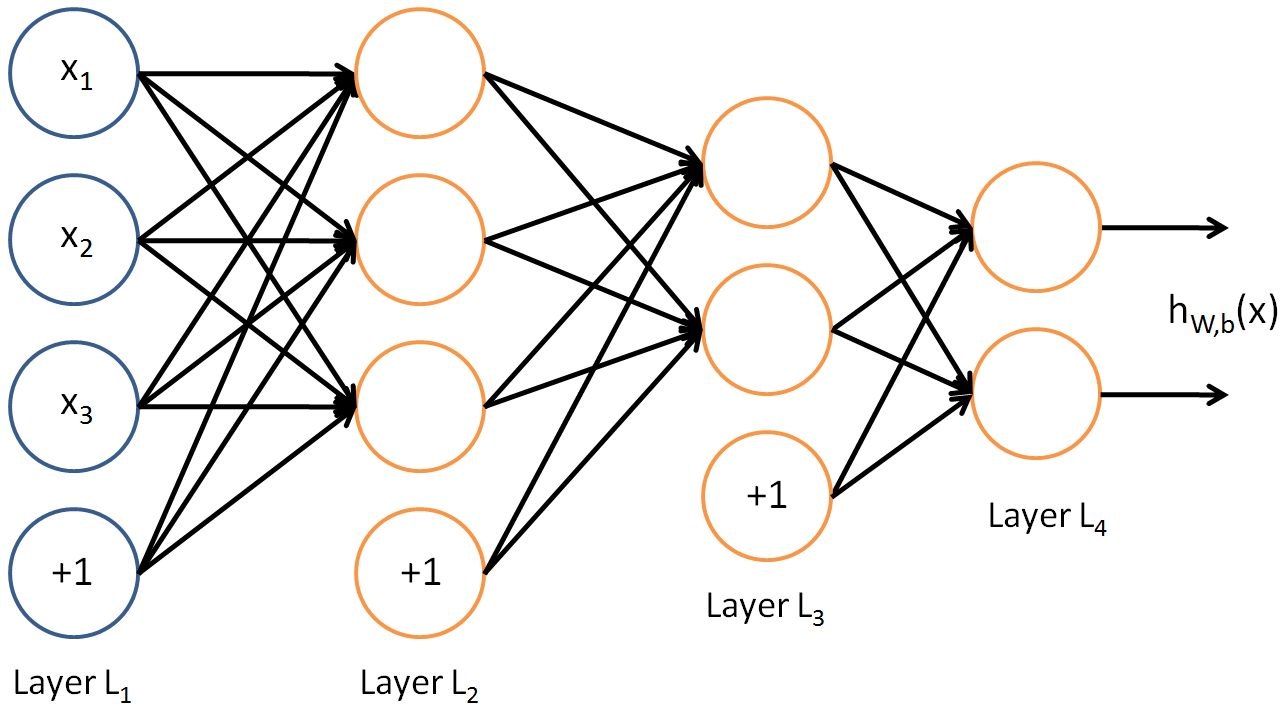
\includegraphics[height=3.2cm]{figs/Network3322.png}
\end{figure}

\item How to train the model with a fixed training set $\{(x^{(1)}, y^{(1)}), \cdots, (x^{(m)}, y^{(m)})\}$ of $m$ training samples?

\end{itemize}
\end{frame}

\begin{frame}
\frametitle{Cost Function}
\begin{itemize}
\item We define the cost function with respect to a single example as a (one-half) squared-error cost function:

\beq{
J(W, b; x, y)=\frac{1}{2}||h_{W,b}(x)-y||^2
}

\item Given a training set of $m$ samples, we then define the overall cost function to be:

\beqn{
J(W, b)=[\frac{1}{m}\sum_{i=1}^{m}J(W, b; x^{(i)}, y^{(i)})]+\frac{\lambda}{2}\sum_{l=1}^{n_l-1}\sum_{i=1}^{s_l}\sum_{j=1}^{s_{l+1}}(W_{ji}^{(l)})^2
%&=&[\frac{1}{m}\sum_{i=1}^{m}(\frac{1}{2}||h_{W,b}(x^{(i)})-y^{(i)}||^2)]+\frac{1}{2}\sum_{l=1}^{n_l-1}\sum_{i=1}^{s_l}\sum_{j=1}^{s_{l+1}}(W_{ji}^{(l)})^2
}

where $\lambda$ is the regularization parameter. 
\end{itemize}
\end{frame}

\begin{frame}
\frametitle{Training}
\begin{itemize}
\item Our goal is to minimize $\mathcal{J}(W, b)$ as a function of $W$ and $b$.

\item We first initialize each parameter $W_{ij}^{(l)}$ and each $b_i^{(l)}$ to a small random value near zero (say according to a $Normal(0, \epsilon^2)$ distribution for some small $\epsilon$).

\item We then apply an optimization algorithm such as batch gradient descent.

\item Since $\mathcal{J}(W,b)$ is a non-convex function, gradient descent is susceptible to local optima; however, in practice gradient descent usually works fairly well. 
\end{itemize}
\end{frame}

\begin{frame}
\frametitle{Training}
\begin{itemize}
\item One iteration of gradient descent updates the parameters $W, b$ as follows:
\beqn{
W_{ij}^{(l)}&=& W_{ij}^{(l)}-\alpha \frac{\partial}{\partial W_{ij}^{(l)}}J(W, b)\\
b_i^{(l)} &=& b_i^{(l)} - \alpha \frac{\partial}{\partial b_i^{(l)}}J(W, b)
}

\item where $\alpha$  is the learning rate. 
\item The key step is computing the partial derivatives above.
\item We next describe the \textbf{backpropagation} algorithm, which gives an efficient way to compute these partial derivatives.
\end{itemize}
\end{frame}

\begin{frame}
\frametitle{Backpropagation: Intuition}
\begin{itemize}
\item Given a training example $(x,y)$, we will first run a ``forward pass'' to compute all the activations throughout the network, including the output value of the hypothesis $h_{W,b}(x)$.
\item Then, for each node $i$ in layer $l$, we would like to compute an ``error term'' $\delta^{(l)}_i$ that measures how much that node was ``responsible'' for any errors in our output. 
\item For an output node, we can directly measure the difference between the network's activation and the true target value, and use that to define $\delta^{(n_l)}_i$. 
\item For hidden units, we will compute $\delta^{(l)}_i$ based on a weighted average of the error terms of the nodes that uses $a^{(l)}_i$ as an input.
\end{itemize}
\end{frame}

\begin{frame}
\frametitle{Backpropagation Algorithm}
\begin{itemize}
\item Perform a forward pass, computing the activations for layers $L_2, L3$, and so on up to the output layer $L_{n_l}$.
\item For each output unit i in layer nl (the output layer), set
\beq{\small
\delta_i^{(n_l)}=\frac{\partial}{\partial z_i^{(n_l)}} \frac{1}{2} ||y-h_{W,b}(x)||^2=-(y_i-a_i^{(n_l)})\cdot f'(z_i^{(n_l)})
}
\item For \tg{$l = n_l-1, n_l-2, \cdots, 2$} and \tb{each node $i$} in layer $l$, set
\beq{\small
\delta_i^{(l)}=(\sum_{j=1}^{s_{l+1}}W_{ji}^{(l)}\delta_j^{(l+1)})f'(z_i^{(l)})
}
\item Compute the desired partial derivatives, which are given as:
\beqn{\small
\frac{\partial}{\partial W_{ij}^{(l)}}J(W, b; x, y) &=& a_j^{(l)}\delta_i^{(l+1)} \\
\frac{\partial}{\partial b_i^{(l)}}J(W, b; x, y) &=& \delta_i^{(l+1)}
}
\end{itemize}
\end{frame}

\begin{frame}
\frametitle{Autoencoder}
\begin{itemize}
\item Previously, we have described the application of neural networks to supervised learning.
\item An autoencoder neural network is an unsupervised learning algorithm that applies backpropagation, setting the target values to be equal to the inputs.

\begin{figure}
      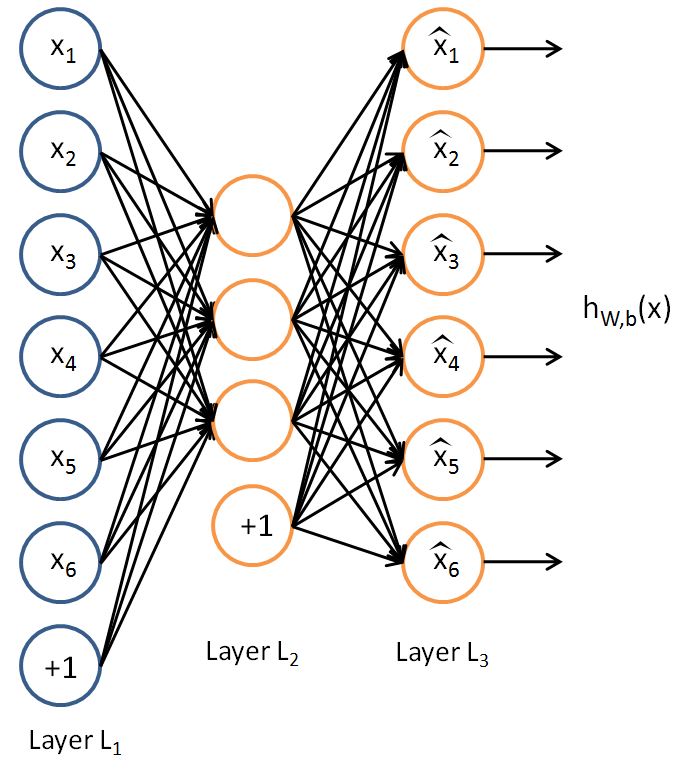
\includegraphics[height=3.8cm]{figs/Autoencoder636.png}
\end{figure}

\item The autoencoder tries to learn a function $h_{W,b}(x) \approx x$.
\end{itemize}
\end{frame}

\begin{frame}
\frametitle{An Example}
\begin{itemize}
\item Suppose the inputs $x$ are the pixel intensity values from a $10 \times 10$ image (100 pixels) so $n=100$.
\item There are $s_2=50$ hidden units in layer $L_2$. 
\item We have $y\in \Re^{100}$.
\item Given only the vector of hidden unit activations $a^{(2)} \in \Re^{50}$, the network must try to reconstruct the 100-pixel input $x$. 
\item Since there are only 50 hidden units, it is forced to learn a \textbf{compressed representation} of the input.  
\item If the input were completely random (e.g., each $x_i$ comes from an IID Gaussian independent of the other features) then this compression task would be very difficult.
\item If there is structure in the data (e.g., some of the input features are correlated),  then this algorithm often ends up learning a \textbf{low-dimensional representation} very similar to PCAs.
\end{itemize}
\end{frame}

\begin{frame}
\frametitle{Sparsity}
\begin{itemize}
\item When the number of hidden units is large (greater than the number of input units), we can still discover interesting structure, by imposing a \textbf{sparsity} constraint on the hidden units. 
\item When considering a sigmoid activation function, we will think of a neuron as being ``active'' if its output value is close to 1, or as being ``inactive'' if its output value is close to 0.
\item We let $\rho_j$ be the average activation of hidden unit $j$ (averaged over the training set).
\beq{
\hat\rho_j = \frac{1}{m} \sum_{i=1}^m \left[ a^{(2)}_j(x^{(i)}) \right]
}
\item Defining a \textbf{sparsity parameter} $\rho$, we would like to (approximately) enforce the constraint
\beq{
\hat\rho_j = \rho,
}
\item Typically $\rho$ has a small value close to zero. To satisfy this constraint, the hidden unit's activations must mostly be near 0.

\end{itemize}
\end{frame}

\begin{frame}
\frametitle{Cost Function}
\begin{itemize}
\item We add an extra penalty term to our optimization objective that penalizes $\hat\rho_j$ deviating significantly from $\rho$. For instance:
\beq{
\sum_{j=1}^{s_2} \rho \log \frac{\rho}{\hat\rho_j} + (1-\rho) \log \frac{1-\rho}{1-\hat\rho_j}.
}
where $s_2$ is the number of neurons in the hidden layer. 

\item This penalty term is based on \tr{KL divergence}, and can also be written
\beq{
\sum_{j=1}^{s_2} {\rm KL}(\rho || \hat\rho_j),
}

where  ${\rm KL}(\rho || \hat\rho_j)
 = \rho \log \frac{\rho}{\hat\rho_j} + (1-\rho) \log \frac{1-\rho}{1-\hat\rho_j}$ is the Kullback-Leibler divergence between two \tb{Bernoulli} random variables with mean $\rho$ and $\hat\rho_j$ respectively.
\end{itemize}
\end{frame}

\begin{frame}
\frametitle{Learning}
\begin{itemize}
\item The overall cost function is now
\beq{
J_{\rm sparse}(W,b) = J(W,b) + \beta \sum_{j=1}^{s_2} {\rm KL}(\rho || \hat\rho_j),
}

%where $J(W,b)$ is as defined previously, and  $\beta$ controls the weight of the sparsity penalty term.
\item  Previously for the second layer ($l=2$), during backpropagation we would have computed
\beq{
\delta^{(2)}_i = \left( \sum_{j=1}^{s_{2}} W^{(2)}_{ji} \delta^{(3)}_j \right) f'(z^{(2)}_i),
}

\item Now instead compute
\beq{
\delta^{(2)}_i =
  \left( \left( \sum_{j=1}^{s_{2}} W^{(2)}_{ji} \delta^{(3)}_j \right)
+ \beta \left( - \frac{\rho}{\hat\rho_i} + \frac{1-\rho}{1-\hat\rho_i} \right) \right) f'(z^{(2)}_i) .
}
\item One subtlety is that you'll need to know $\hat\rho_i$ to compute this term.

\end{itemize}
\end{frame}

\begin{frame}
\frametitle{Implementation Notes}
\begin{itemize}
\item Before computing backpropagation on any example, we compute a forward pass on all the training examples first to compute the average activations on the training set. 
\item If the training set is small enough to fit comfortably in computer memory, we can compute forward passes on all your examples and keep the resulting activations in memory and compute the $\hat\rho_i$s. 
\end{itemize}
\end{frame}

\begin{frame}
\frametitle{Implementation Notes}
\begin{itemize}
\item If the data is too large to fit in memory, we may have to scan through the examples computing a forward pass on each to accumulate the activations and compute $\hat\rho_i$ (discarding the result of each forward pass after you have taken its activations $a^{(2)}_i$ into account for computing $\hat\rho_i$). 
\item After having computed $\hat\rho_i$, we have to redo the forward pass for each example so that we can do backpropagation on that example. 
\item We compute a forward pass twice on each training example, making it computationally less efficient.
\end{itemize}
\end{frame}

\begin{frame}
\frametitle{Visualizing a Trained Autoencoder}
\begin{itemize}
\item We have a trained sparse autoencoder with 100 hidden units on $10 \times 10$ pixel inputs.

\item We visualize 100 images (one per hidden unit) and try to understand what the ensemble of hidden units is learning.
\begin{figure}
      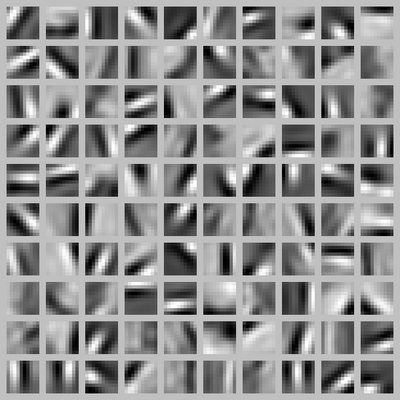
\includegraphics[height=3.8cm]{figs/ExampleSparseAutoencoderWeights.png}
\end{figure}

\item Each square in the figure above shows the (norm bounded) input image $x$ that maximally actives one of 100 hidden units. 

\item Different hidden units have learned to detect edges at different positions and orientations in the image.
\end{itemize}
\end{frame}

\section{Restricted Boltzmann Machine}

\begin{frame}
  \frametitle{Contents}
  \tableofcontents[currentsection]
\end{frame}

\begin{frame}
\frametitle{Energy-Based Models (EBM)}
\begin{itemize}
\item 
Energy-based probabilistic models define a probability distribution through an energy function, e.g.:
\begin{equation}
P(x)=\frac{\exp(-E(x))}{Z}
\end{equation}
Here $p(x)$ is also called a \tr{Boltzmann distribution} (or \tb{Gibbs distribution}).
\item 
EBMs with Hidden Units:
\begin{equation}
P(x)=\sum_h P(x, h)=\sum_h \frac{\exp(-E(x,h))}{Z}
\end{equation}
\item 
Formulation with \textbf{free energy}:
\begin{eqnarray}
F(x)&=&-\log \sum_h \exp(-E(x, h))\\
P(x)&=&\frac{\exp(-F(x))}{Z}
\end{eqnarray}
\end{itemize}

\end{frame}

%------------------------------------------------

\begin{frame}
\frametitle{General Boltzmann Machine}
\begin{itemize}
\item A BM is a particular type of MRF that has a two-layer architecture.
\item Random variables $\mathbf{x} \in \{0, 1\}$ are observed, $\mathbf{h} \in \{0, 1\}$ are hidden. 
\item Their joint is given by the Boltzmann distribution associated with an energy function $E(\mathbf{x}, \mathbf{h})$:
\begin{equation}\small
P(\mathbf{x, h}) = \frac{\exp(-E(\mathbf{x, h}))}{Z}
\end{equation}
\item Let $\mathbf{z}=(\mathbf{x}, \mathbf{h})$, the energy function is a quadratic polynomial:
\begin{equation}\small
E(\mathbf{z})=-\sum_i b_i z_i - \sum_{ij} w_{ij}z_iz_j
\end{equation}
\end{itemize}
\begin{figure}
\centering
  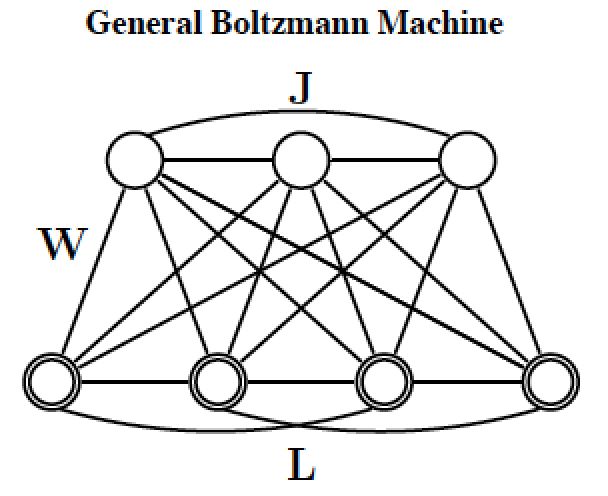
\includegraphics[width=0.32\textwidth]{figs/bm.png}
  %\caption{Restricted Boltzmann Machine.}
  %\vspace{-0.1in}
%\vspace{-0.1in}	
\end{figure}
\end{frame}

%------------------------------------------------

\begin{frame}
\frametitle{Parameter Estimation}
\begin{itemize}
\item The likelihood involves a sum over all configurations of $\mathbf{h}$:
\begin{equation}
P(\mathbf{x}|\mathbf{h}) = \sum_{\mathbf{h}}P(\mathbf{x, h})=\sum_{\mathbf{h}}\frac{\exp(-E(\mathbf{x, h}))}{Z}
\end{equation}
\item The gradient of $\log P(\mathbf{x})$ wrt $\theta=\{b, w\}$:
\begin{eqnarray}
\frac{\partial P(\mathbf{x})}{\partial \theta}&=&\sum_{\mathbf{h}}P(\mathbf{h}|\mathbf{x}) \frac{\partial E(\mathbf{h,x})}{\partial \theta}-\sum_{\mathbf{x, h}}P(\mathbf{x, h})\frac{\partial E(\mathbf{x, h})}{\partial \theta}\\
&=&\mathbb{E}_{P_{data}}[\frac{\partial E(\mathbf{x,h})}{\partial \theta}]-\mathbb{E}_{P_{model}}[\frac{\partial E(\mathbf{x, h})}{\partial \theta}]
\end{eqnarray}
\item Unfortunately, both \textit{data-dependent expectation} and \textit{model-dependent expectation} are intractable for General Boltzmann Machine.
\end{itemize}
\end{frame}

%------------------------------------------------

\begin{frame}
\frametitle{Estimate the Data-Depedent Expectations}
\begin{itemize}
\item Variational learning uses an approximate posterior $Q(\mathbf{h}|\mathbf{x};\mu)$ to replace the true posterior distribution $P(\mathbf{h}|\mathbf{x};\theta)$ and estimates the parameters to maximize the variational lower bound on the log-likelihood:
\beal{
\log P(\mathbf{x};\theta) &\geq \sum_h Q(\mathbf{h}|\mathbf{x};\mu) \log P(\mathbf{x}, \mathbf{h}; \theta) + H(Q)\\
&= \log P(\mathbf{x}; \theta) - KL[Q(\mathbf{h}|\mathbf{x};\mu) || P(\mathbf{h}|\mathbf{x};\theta)]
}
where $H(\cdot)$ is the entropy function. 

\end{itemize}
\end{frame}

%------------------------------------------------

\begin{frame}
\frametitle{Estimate the Data-Depedent Expectations (cont.)}
\begin{itemize}
\item We approximate the true posterior by a fully factorized distribution: $Q(\mathbf{h};\mu)=\prod_{i=1}^{F}q(h_i)$, with $q(h_i=1)=\mu_i$ and $F$ is the number of hidden units.
\item Energy function: $E(\mathbf{x, h})=-\frac{1}{2}\mathbf{x}^T\mathbf{L}\mathbf{x}-\frac{1}{2}\mathbf{h}^T\mathbf{J}\mathbf{h}-\mathbf{x}^T\mathbf{W}\mathbf{h}$ 
\item The new lower bound:
\beal{
\log P(\mathbf{x};\theta) &\geq \frac{1}{2} \sum_{i,k} L_{ik}x_ix_k+\frac{1}{2}\sum_{j,m}J_{jm}\mu_j\mu_m+\sum_{i,j}W_{ij}x_i\mu_j\\
&-\log Z(\theta)+\sum_j[\mu_j\log \mu_j+(1-\mu_j)\log(1-\mu_j)] \nonumber
}

\item The learning proceeds first maximizes this lower bound with respect to the variational parameters $\mathbf{\mu}$ for fixed $\mathbf{\theta}$:
\begin{equation}
\mu_j \leftarrow g(\sum_i W_{ij}x_i+\sum_{m \neq j}J_{mj}\mu_m)
\end{equation}
where $g(\cdot)$ is the logistic function.
\end{itemize}
\end{frame}

%------------------------------------------------

\begin{frame}
\frametitle{Estimate the Model-Depedent Expectations}
\begin{itemize}
\item Unfortunately, variational approach cannot be used for approximating the expectations with respect to the model distribution in RBM [Galland, 1991]
\item We use Gibbs sampling to approximate the intractable model's expectation $\mathbb{E}_{P_{model}}[\cdot]$ (see details in RBM section). 
\end{itemize}
\end{frame}

%------------------------------------------------

\begin{frame}
\frametitle{Learning Procedure}
\begin{figure}
\centering
  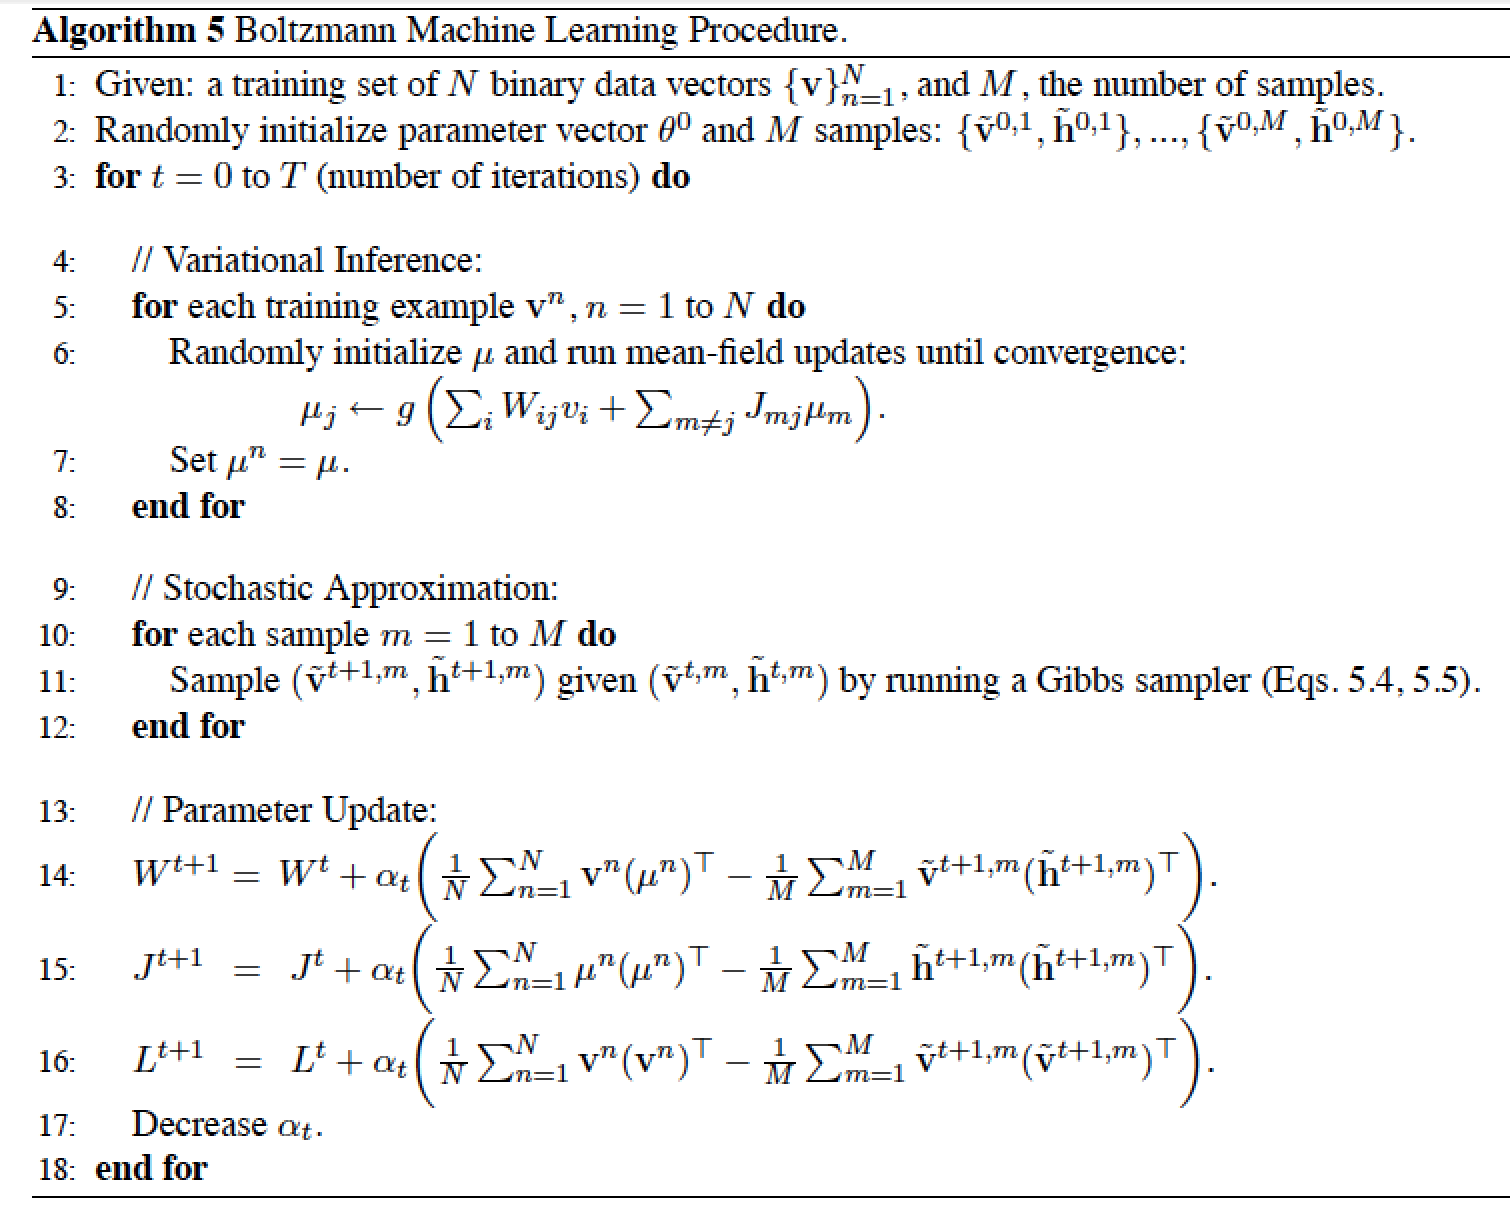
\includegraphics[width=0.8\textwidth]{figs/learning.png}
  %\caption{Gibbs sampling in RBM.}
  %\vspace{-0.1in}
%\vspace{-0.1in}	
\end{figure}
\end{frame}

%------------------------------------------------

\begin{frame}
\frametitle{Restricted Boltzmann Machine}
\begin{itemize}
\item A RBM is a particular type of MRF that has a two-layer architecture.
\item Visible stochastic units $\mathbf{v} \in \{0, 1\}^D$ are connected to hidden units $\mathbf{h} \in \{ 0, 1\}^F$.
\item The energy of the state $\{\mathbf{v}, \mathbf{h}\}$ is
\begin{equation}
E(\mathbf{v, h; \theta}) = -\mathbf{v}^T W \mathbf{h} - \mathbf{b}^T\mathbf{v} - a^T\mathbf{h}
\end{equation}
\item We have the joint distribution over the visible and hidden units as follows
\begin{equation}
P(\mathbf{v, h}; \theta) = \frac{1}{Z(\theta)}\exp\{-\mathbb{E}(\mathbf{v, h}; \theta)\}
\end{equation}
\end{itemize}
\begin{figure}
\centering
  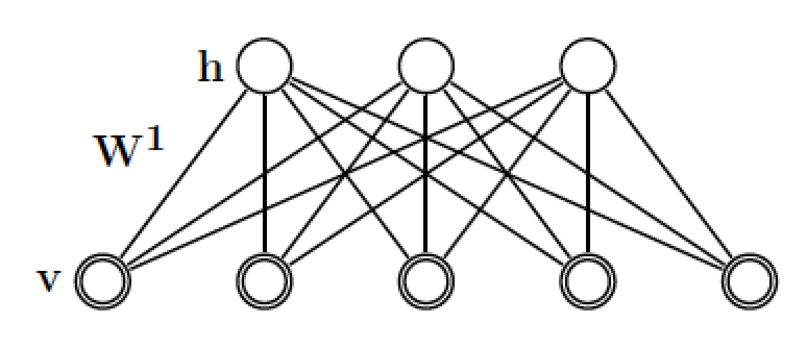
\includegraphics[width=0.4\textwidth]{figs/rbm_model.pdf}
  \caption{Restricted Boltzmann Machine.}
  %\vspace{-0.1in}
%\vspace{-0.1in}	
\end{figure}
\end{frame}

%------------------------------------------------

\begin{frame}
\frametitle{Inference: $p(h|v)$}

\begin{eqnarray}
p(h|v) & = & \frac{p(h, v)}{\sum_{h'}p(h', v)} \\ \pause 
& = & \frac{exp(v^TWh+b^Tv+a^Th)/Z(\theta)}{\sum_{h'}exp(v^TWh'+b^Tv+a^Th)/Z(\theta)} \\ \pause 
& = & \frac{exp(v^TWh+a^Th)}{\sum_{h'}exp(v^TWh'+a^Th)} \\ \pause 
& = & \frac{\prod_{j}exp(h_jW_jv+a_jh_j)}{\sum_{h'}\prod_{j}exp(h'_jW_jv+a_jh'_j)}\\ \pause 
& = & \frac{\prod_{j}exp(h_jW_jv+a_jh_j)}{\prod_{j} (\sum_{h' \in \{0, 1\}}exp(h'_jW_jv+a_jh'_j))}\\ \pause 
& = & \prod_j \frac{exp(h_jW_jv+a_jh_j)}{1+exp(W_jv+a_j)} \\ \pause 
& = & \prod_j p(h_j|v)
\end{eqnarray}

\end{frame}

%------------------------------------------------

\begin{frame}
\frametitle{Inference: $p(h=1|v)$}

\begin{eqnarray}
p(h|v) & = & \frac{exp(W_jv+a_j)}{1+exp(W_jv+a_j)} \\ \pause
& = & \frac{1}{1+exp(-W_jv-a_j)} \\ \pause
& = & g(W_jv+a_j) 
\end{eqnarray}

\noindent \ \ \ \ \ \ \ \ \ \ \ \ \ \ \ \ \ \ \ \ \ \ \ \ \ \ \ \ \  where $g(\cdot)$ is the logistic function.

\end{frame}

%------------------------------------------------


\begin{frame}
\frametitle{Summary}
\begin{itemize}
\item We have the joint distribution over the visible and hidden units as follows
\begin{equation}
P(\mathbf{v, h}; \theta) = \frac{1}{Z(\theta)}\exp\{-\mathbb{E}(\mathbf{v, h}; \theta)\}
\end{equation}
\item The hidden units can be marginalized out to get the probability of a visible vector $\mathbf{v}$:
\begin{equation}
P(\mathbf{v}; \theta)=\frac{1}{Z(\theta)}\exp(\mathbf{b}^T\mathbf{v})\prod_{j=1}^{F}(1+\exp(\alpha_j+\sum_{d=1}^{D}W_{ij}v_i))
\end{equation}
\item The conditional distributions over hidden units and visible vector can be derived from the equations above
\begin{equation}
p(h_j=1|v) = g(\sum_i W_{ij}v_i+\alpha_j)
\end{equation}
\begin{equation}
p(v_i=1|h) = g(\sum_j W_{ij}h_j+\beta_i)
\end{equation}
\noindent where $g(\cdot)$ is the logistic function.
\end{itemize}
\end{frame}

%------------------------------------------------

\begin{frame}
\frametitle{Model Learning (Stochastic Gradient Descent)}
\begin{figure}
\centering
  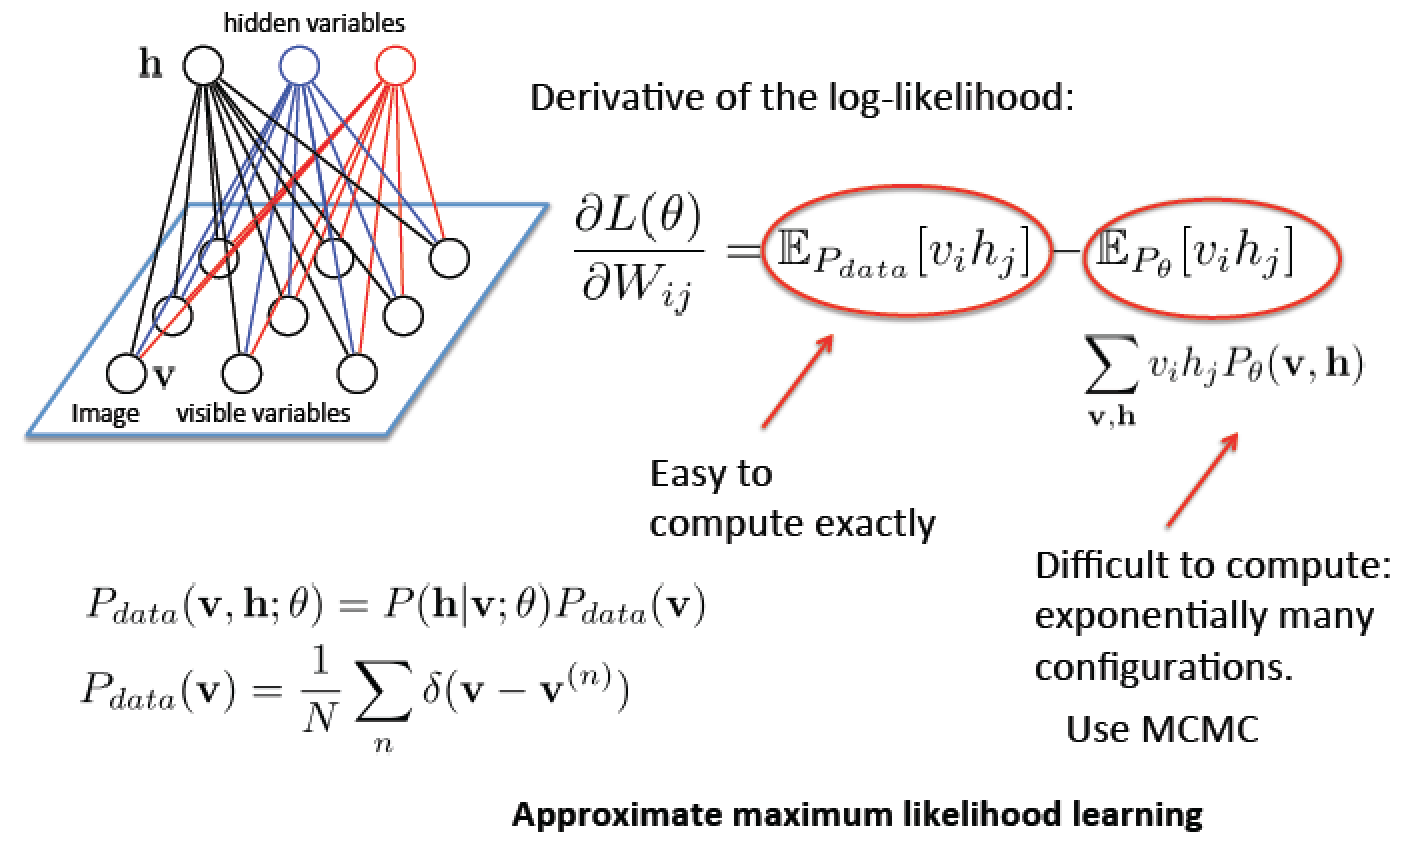
\includegraphics[width=0.8\textwidth]{figs/rbm_estimate.png}
  %\vspace{-0.1in}
%\vspace{-0.1in}	
\end{figure}
\end{frame}

%------------------------------------------------

\begin{frame}
\frametitle{Constrative Divergence}
\begin{itemize}
\item The first practical method for training RBMs proposed by Hinton in 2002.
\item Main idea: the \tr{model-dependent expectation} (also known as negative gradiant) can be approximated using samples obtained by starting a Gibbs chain at a training vector.
\item CD learning has been used extensively for training RBMs and other energy-based models. 
\end{itemize}
\end{frame}

\begin{frame}
\frametitle{Details of Constrative Divergence}
\begin{itemize}
\item Gibbs sampling of the joint of N random variables $S=(S_1, \dots, S_N)$ is done through a sequence of N sampling sub-steps of the form $S_i \sim p(S_i|S_{-i})$ where $S_{-i}$ contains the N-1 other random variables in $S$ excluding $S_i$.
\item For RBMs, $S$ consists of visible and hidden units, which are conditional independent. A step in the Markov chain is thus taken as
\begin{eqnarray}
h^{n+1}&\sim& g(W^Tv^n+\alpha) \\
v^{n+1}&\sim & g(W^Th^{n+1}+\beta)
\end{eqnarray}
\item The sampling process can be illustrated graphically:
\begin{figure}
\centering
  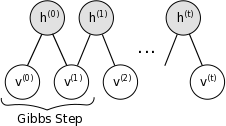
\includegraphics[width=0.3\textwidth]{figs/markov_chain.png}
  \caption{Gibbs sampling in RBM.}
  %\vspace{-0.1in}
%\vspace{-0.1in}	
\end{figure}
\end{itemize}
\end{frame}

%------------------------------------------------

\hide{
\begin{frame}
\frametitle{Persistent CD (PCD)}
\begin{itemize}
\item Persistent contrastive divergence
\begin{itemize}
\item Idea: instead of initializing the chain to $v^{n}$ initialize the chain to the negative sample of the last iteration.
\end{itemize}
\begin{figure}
\centering
  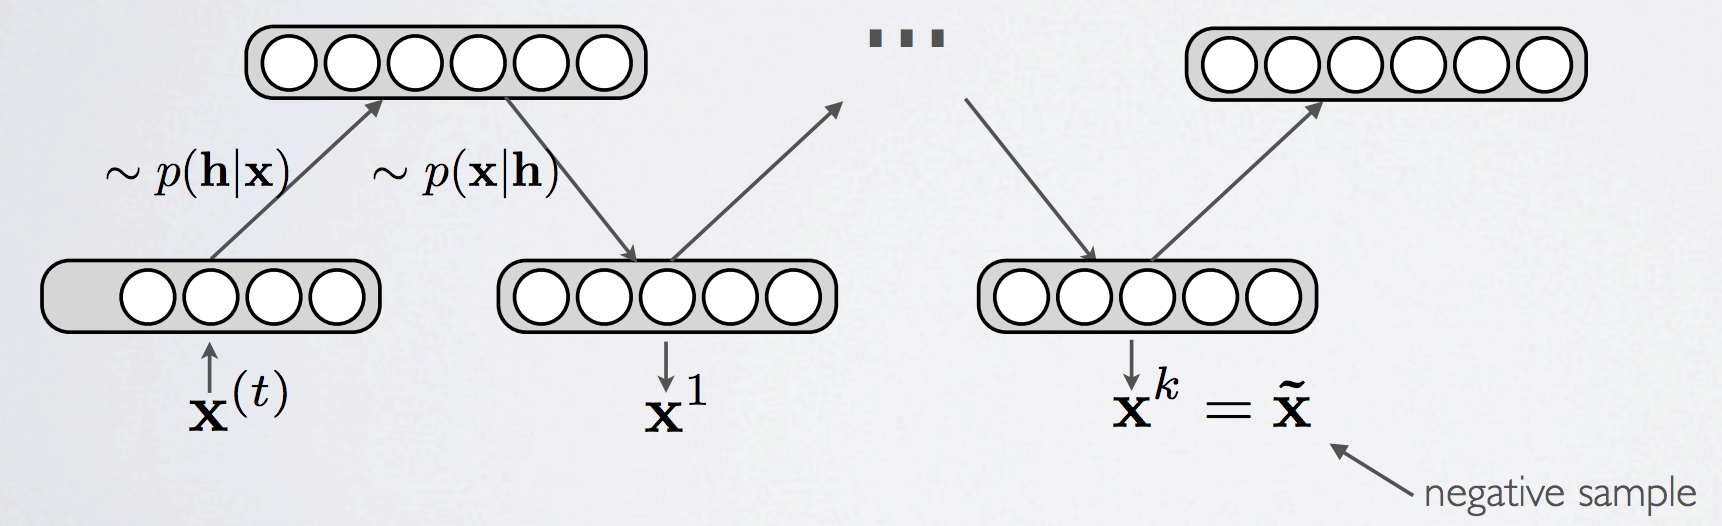
\includegraphics[width=0.8\textwidth]{figs/pcd.png}
  %\caption{Gibbs sampling in RBM.}
  %\vspace{-0.1in}
%\vspace{-0.1in}	
\end{figure}

\end{itemize}
\end{frame}
}
%------------------------------------------------

\begin{frame}
\frametitle{Persistent Contrastive Divergence}
\begin{itemize}
\item One problem with CD learning is that it provides biased
estimates of the gradient.
\item Instead of running a new chain for each parameter update, PCD maintains a single persistent
chain.
\item The update at time $t$ takes the state of the Gibbs chain at time $t-1$, performs one round
of Gibbs sampling, and uses this state in the negative gradient estimates. 
\end{itemize}
\begin{figure}
\centering
  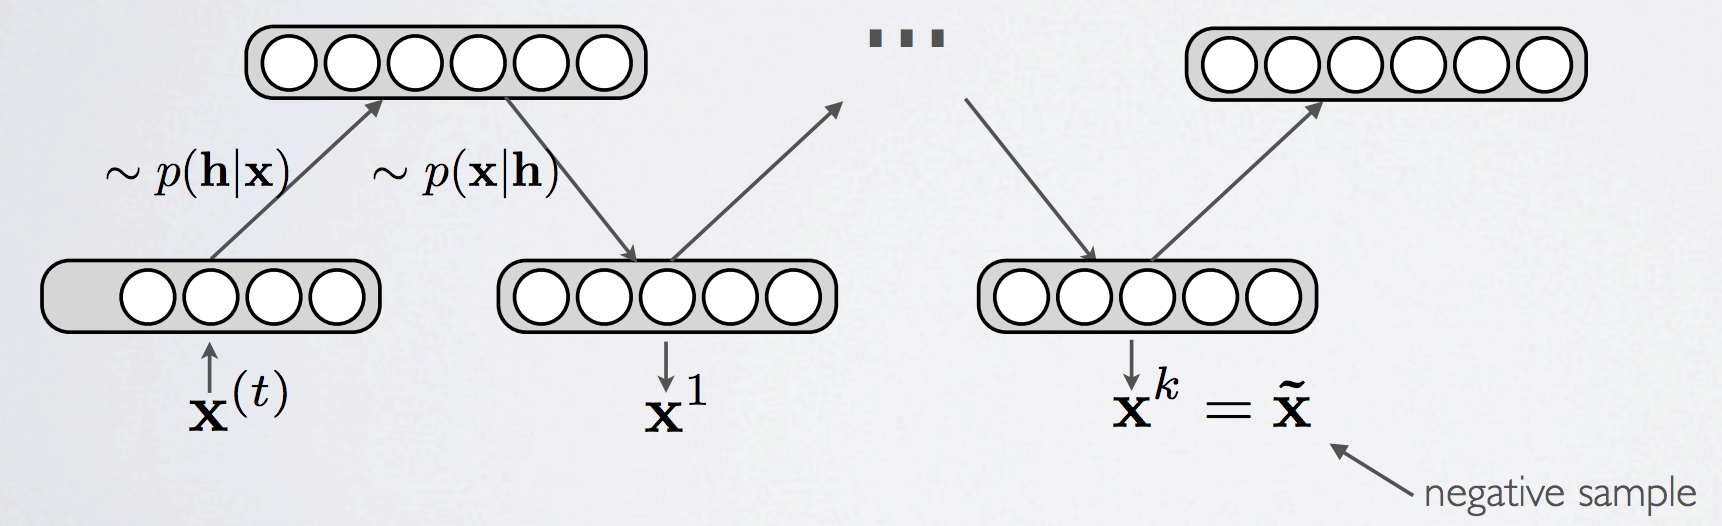
\includegraphics[width=0.8\textwidth]{figs/pcd.png}
  %\caption{Gibbs sampling in RBM.}
  %\vspace{-0.1in}
%\vspace{-0.1in}	
\end{figure}
\end{frame}

%------------------------------------------------

\begin{frame}
\frametitle{Conditional Restrited Boltzmann Machine (CRBM)}
\begin{itemize}
\item A CRBM models the distribution $p(v|u)$ by using an RBM to model $v$ and using $u$ to dynamically
determine the biases or weights of that RBM. 
\item Energy function of the CRBM:
\begin{equation}
E(\mathbf{v, h, u})=-\mathbf{v}^T\mathbf{W}^{vh}\mathbf{h}-\mathbf{b}^T\mathbf{v}-\mathbf{a}^T\mathbf{h}-\mathbf{u}^T\mathbf{W}^{uv}\mathbf{v}-\mathbf{u}^T\mathbf{W}^{uh}\mathbf{h}
\end{equation}
%\item While RBMs have primarily been used for learning new representations of data, conditional RBMs are generally used for making predictions.
\begin{figure}
\centering
  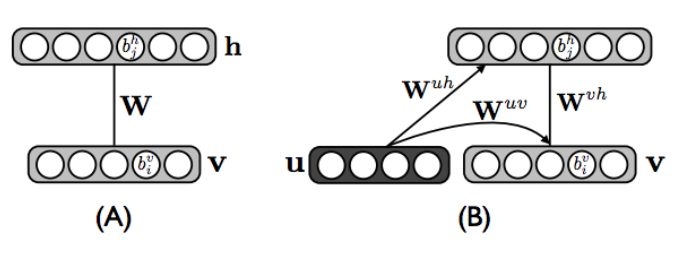
\includegraphics[width=0.7\textwidth]{figs/crbm.png}
  \caption{Illustration of an RBM (A) and a conditional
  RBM (B).}
  %\vspace{-0.1in}
%\vspace{-0.1in}	
\end{figure}
\end{itemize}
\end{frame}

\begin{frame}
\frametitle{Conditional Restrited Boltzmann Machine (CRBM)}
\begin{itemize}

\item The CRBM extends the RBMs to capture temporal dependencies.
\item Does not change inference and learning.
\begin{figure}
\centering
  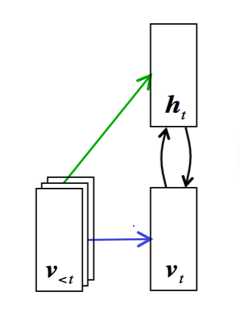
\includegraphics[width=0.3\textwidth]{figs/crbm2.png}
  %\caption{}
  %\vspace{-0.1in}
%\vspace{-0.1in}	
\end{figure}
\end{itemize}
\end{frame}

\begin{frame}
\frametitle{Deep Boltzmann Machine}
\begin{itemize}
\item Consider a three-hidden-layer Boltzmann machine, with no within layer connections. The energy of the state $\{\mathbf{v, h^1, h^2, h^3} \}$is defined as:
\begin{equation}
E(\mathbf{v, h^1, h^2, h^3}; \theta)=-\mathbf{v}^T\mathbf{W}^1\mathbf{h}^1-\mathbf{h}^{1T}\mathbf{W}^2\mathbf{h}^2-\mathbf{h}^{2T}\mathbf{W}^3\mathbf{h}^3
\end{equation}
where $\theta=\{\mathbf{W}^1, \mathbf{W}^2, \mathbf{W}^3\}$ are the model parameters, representing visible-to-hidden and hidden-to-hidden symmetric interaction terms.
\begin{figure}
\centering
  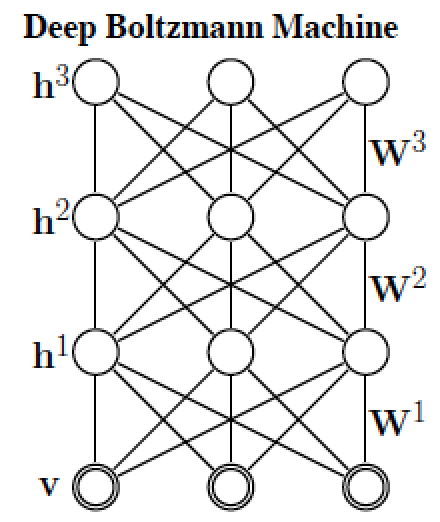
\includegraphics[width=0.3\textwidth]{figs/dbms.png}
  %\caption{Gibbs sampling in RBM.}
  %\vspace{-0.1in}
%\vspace{-0.1in}	
\end{figure}
\end{itemize}
\end{frame}

%------------------------------------------------

\begin{frame}
\frametitle{Deep Boltzamann Machines (cont.)}
\begin{itemize}
\item The probability that the model assigns to a visible vector $\mathbf{v}$ is:
\begin{equation}
P(\mathbf{v};\theta)=\frac{\sum_{\mathbf{h^1,h^2,h^3}}\exp(-E(\mathbf{v, h^1, h^2, h^3};\theta))}{Z(\theta)}
\end{equation}
\item The conditional distributions over the visible and the three sets of hidden units are given by logistic functions:
\begin{figure}
\centering
  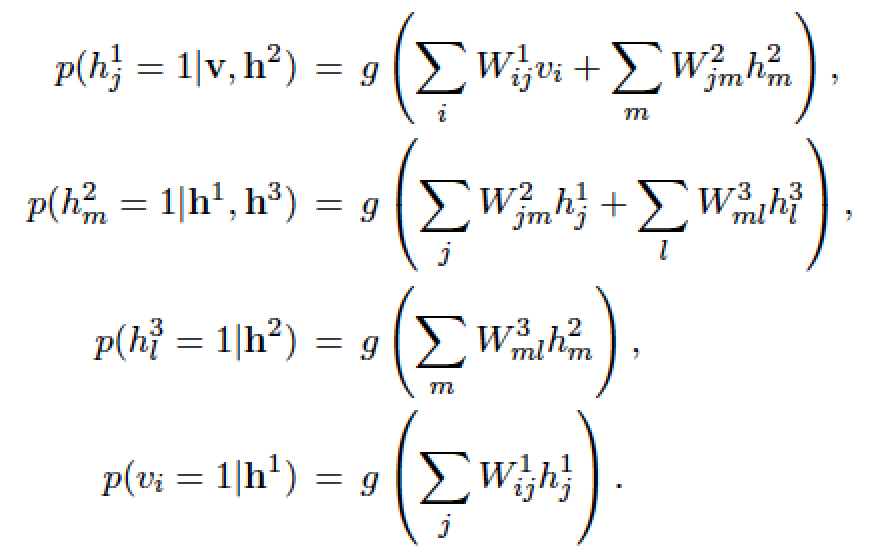
\includegraphics[width=0.55\textwidth]{figs/dbm_update.png}
  %\caption{Gibbs sampling in RBM.}
  %\vspace{-0.1in}
%\vspace{-0.1in}	
\end{figure}
\end{itemize}
\end{frame}

%------------------------------------------------

\begin{frame}
\frametitle{Deep Boltzamann Machines (cont.)}
\begin{figure}
\centering
  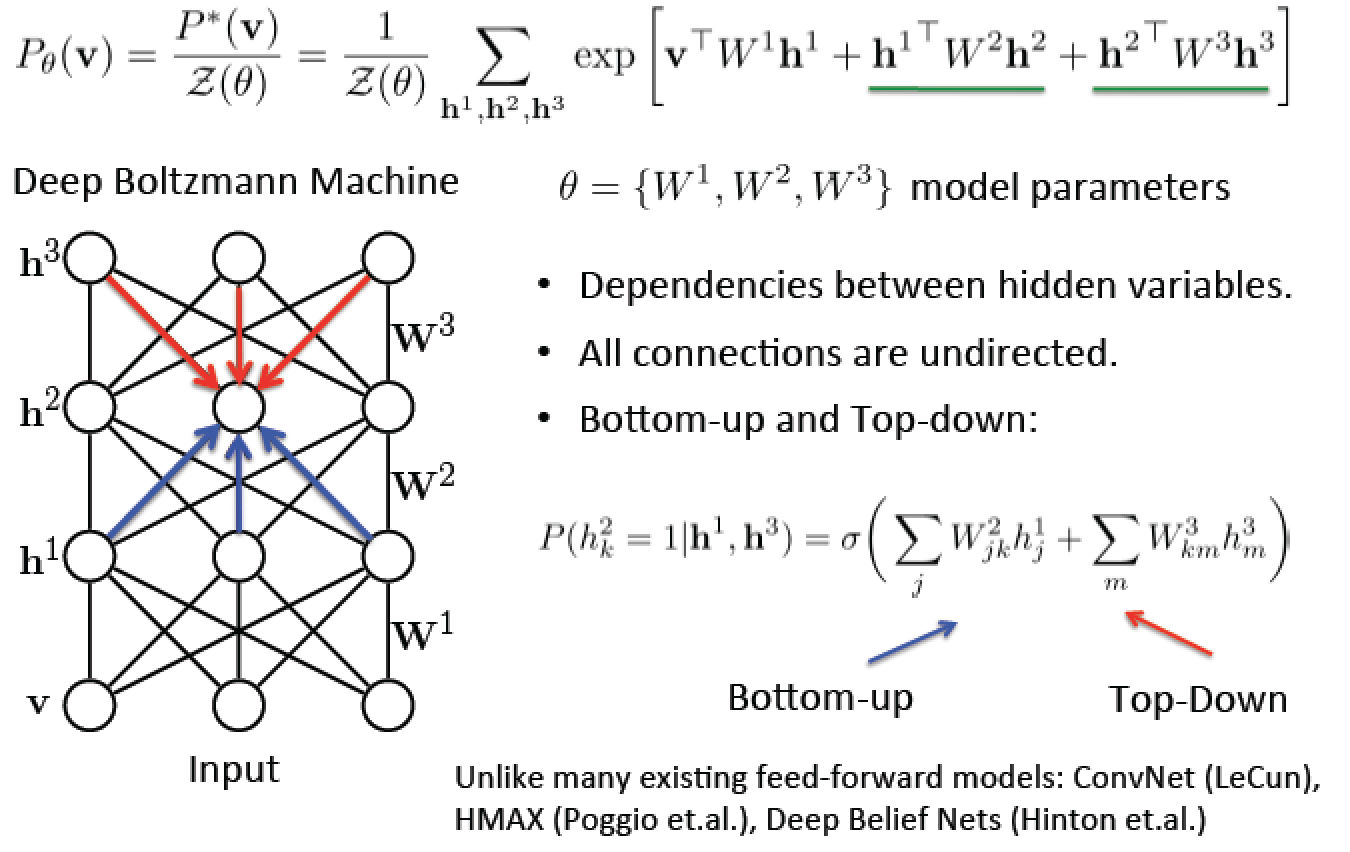
\includegraphics[width=0.8\textwidth]{figs/p1.png}
  %\caption{Gibbs sampling in RBM.}
  %\vspace{-0.1in}
%\vspace{-0.1in}	
\end{figure}
\end{frame}

%------------------------------------------------

\begin{frame}
\frametitle{Deep Boltzamann Machines (cont.)}
\begin{figure}
\centering
  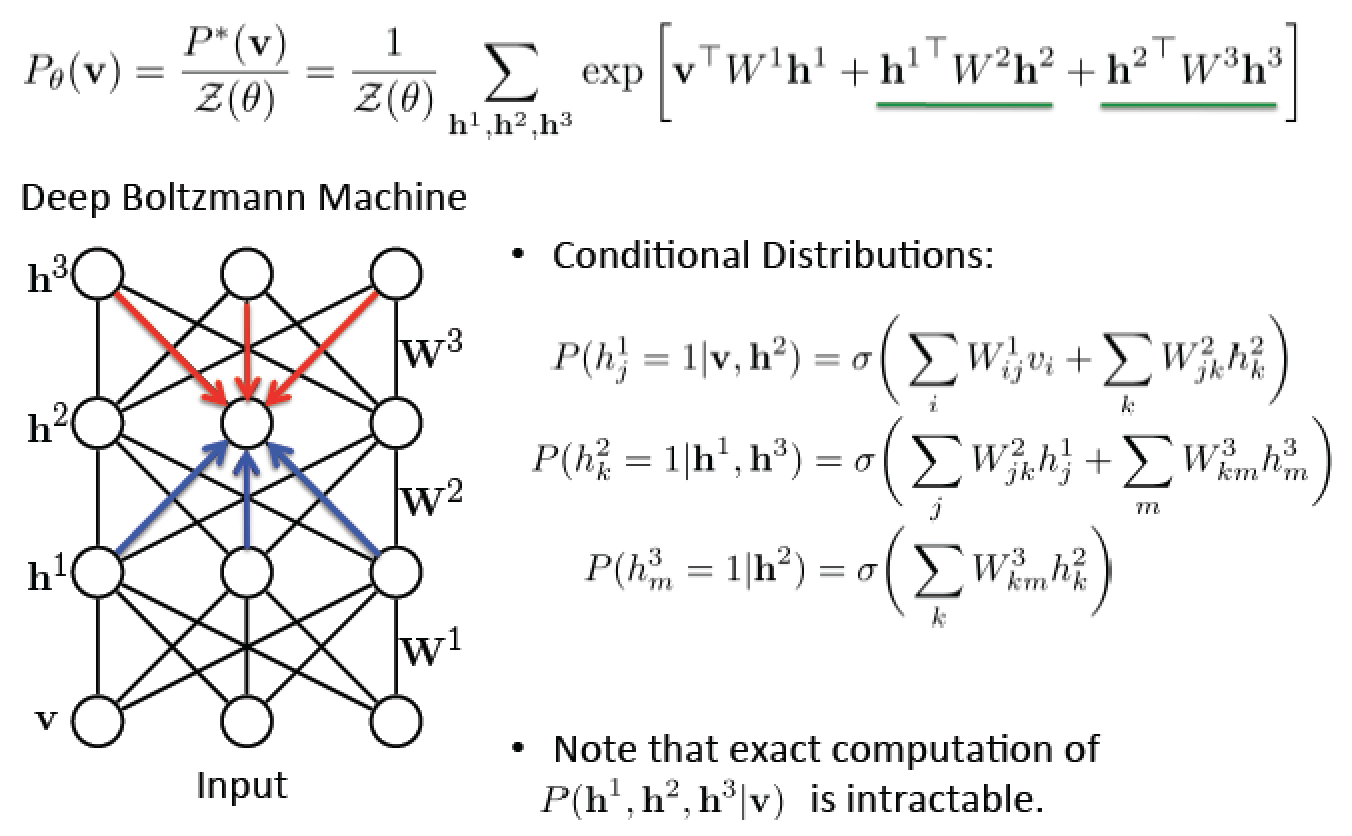
\includegraphics[width=0.8\textwidth]{figs/p2.png}
  %\caption{Gibbs sampling in RBM.}
  %\vspace{-0.1in}
%\vspace{-0.1in}	
\end{figure}
\end{frame}

%------------------------------------------------

\begin{frame}
\frametitle{Deep Boltzamann Machines (cont.)}
\begin{figure}
\centering
  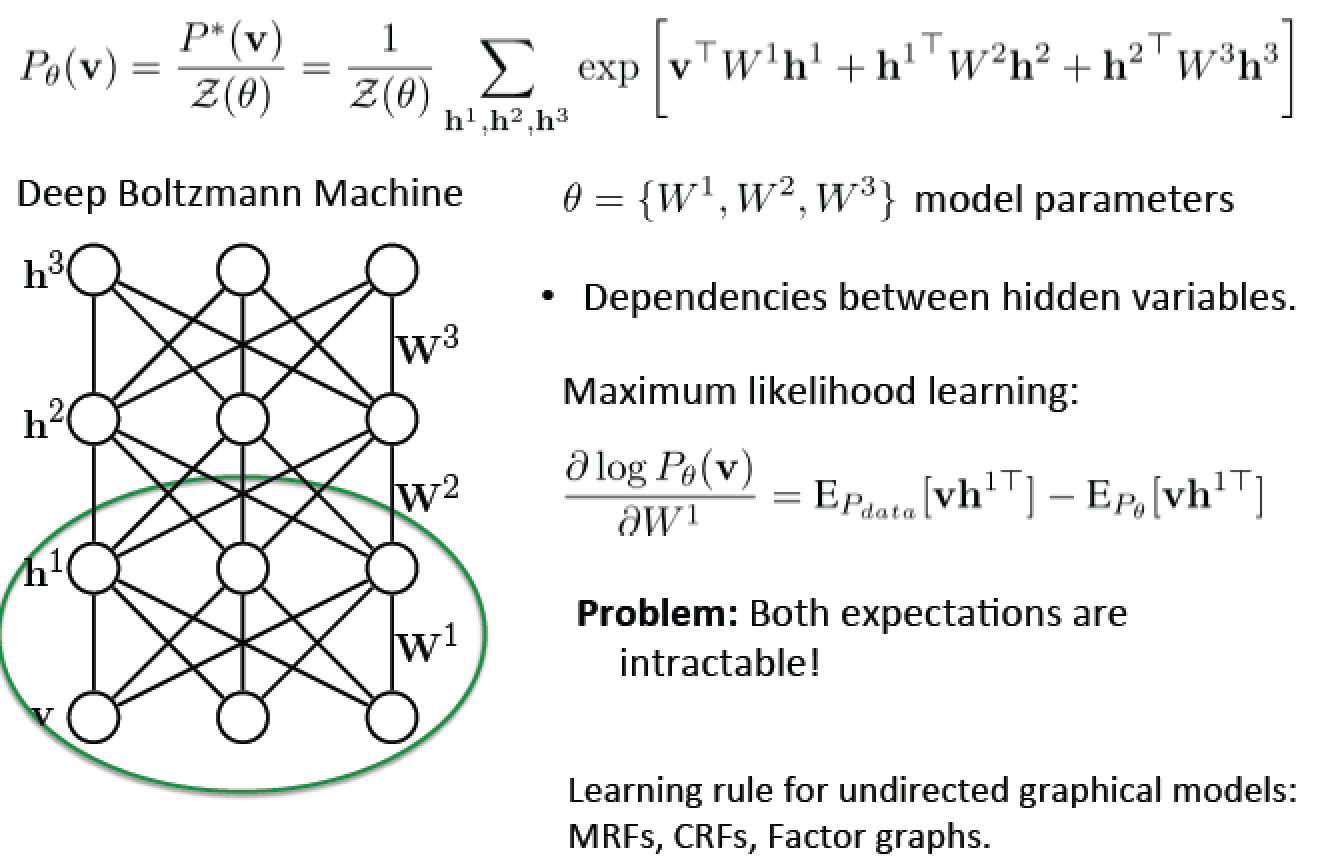
\includegraphics[width=0.8\textwidth]{figs/p3.png}
  %\caption{Gibbs sampling in RBM.}
  %\vspace{-0.1in}
%\vspace{-0.1in}	
\end{figure}
\end{frame}

%------------------------------------------------

\begin{frame}
\frametitle{Deep Boltzamann Machines (cont.)}
\begin{figure}
\centering
  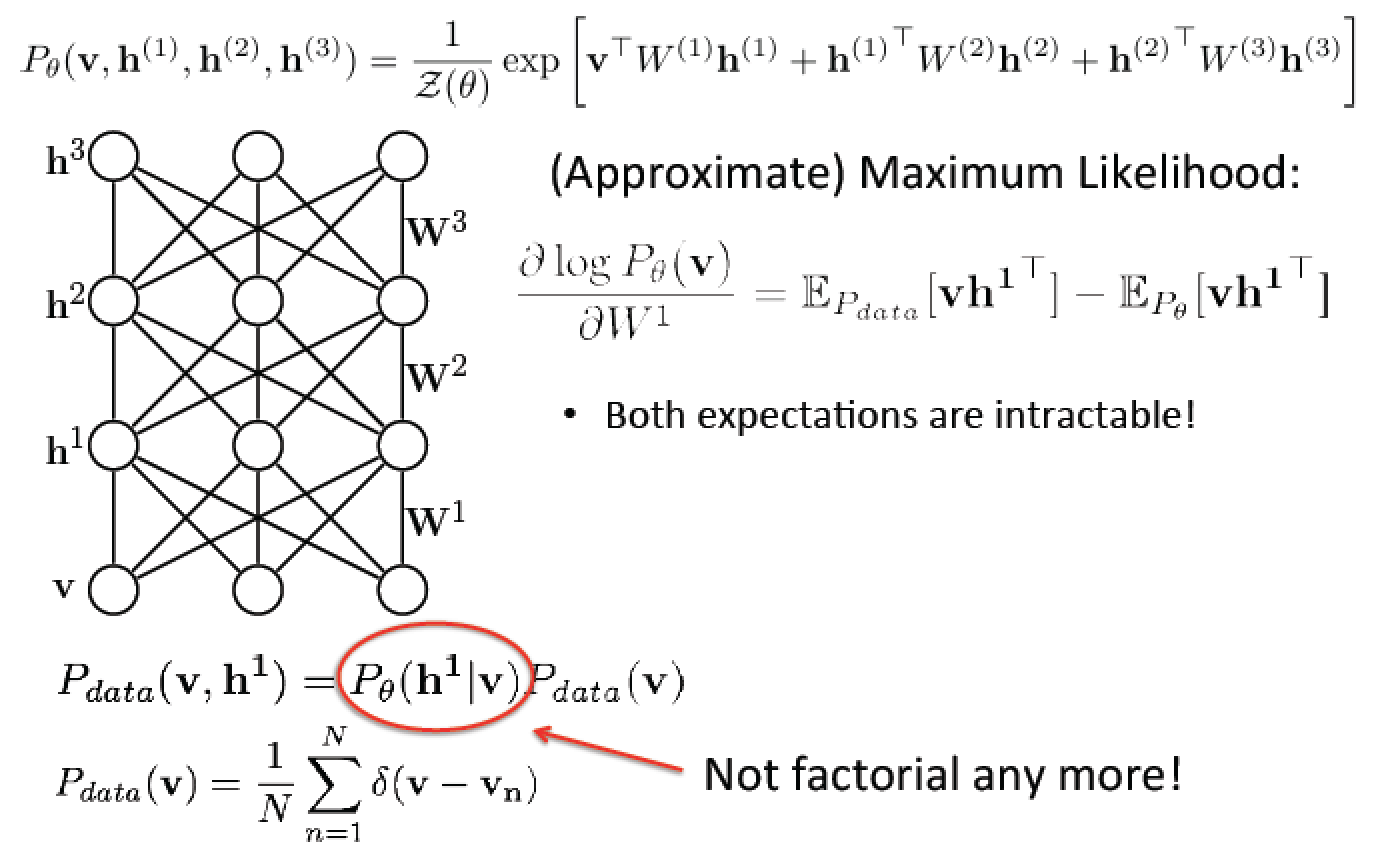
\includegraphics[width=0.8\textwidth]{figs/p4.png}
  %\caption{Gibbs sampling in RBM.}
  %\vspace{-0.1in}
%\vspace{-0.1in}	
\end{figure}
\end{frame}

%------------------------------------------------

\begin{frame}
\frametitle{Deep Boltzamann Machines (cont.)}
\begin{figure}
\centering
  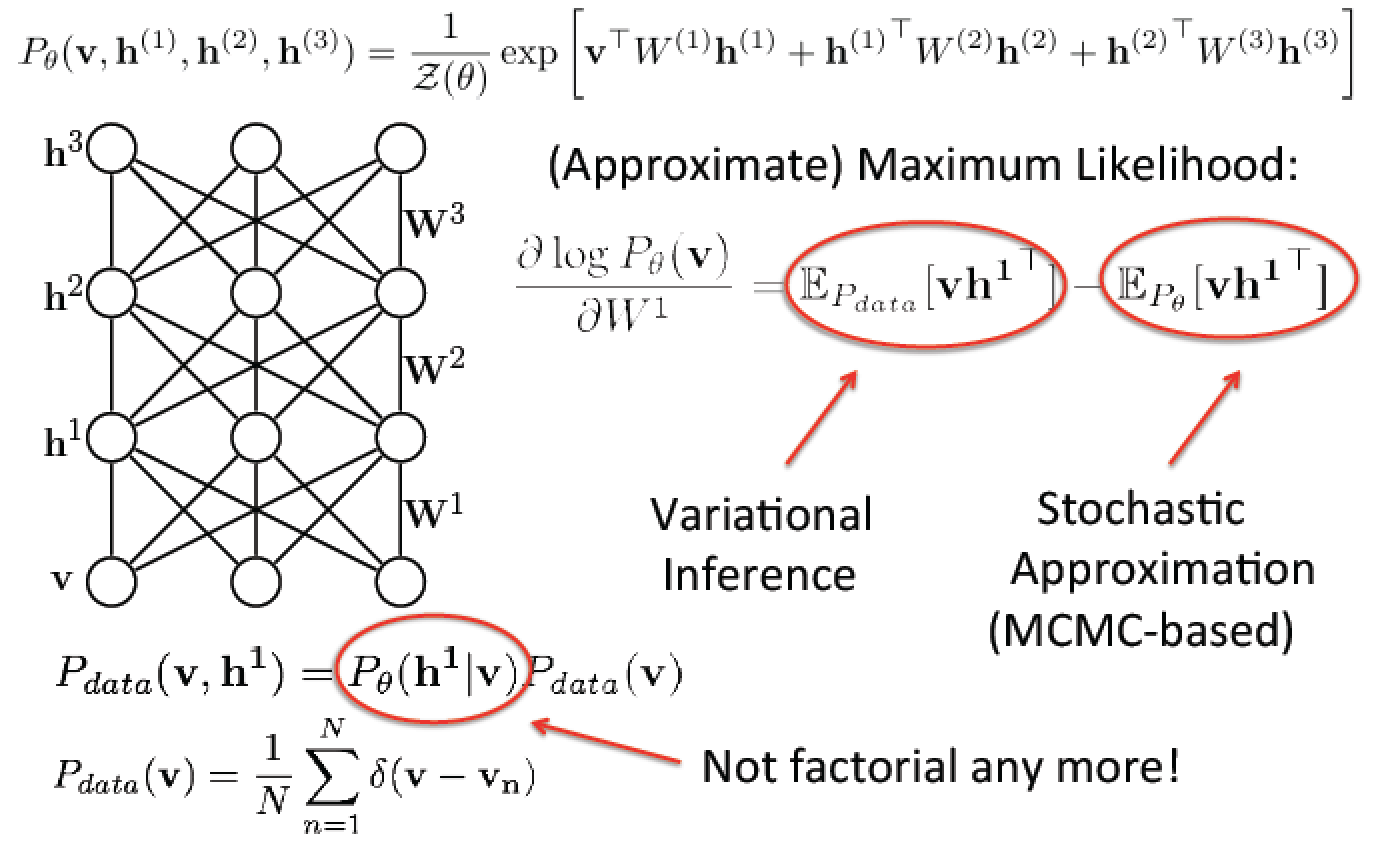
\includegraphics[width=0.8\textwidth]{figs/p5.png}
  %\caption{Gibbs sampling in RBM.}
  %\vspace{-0.1in}
%\vspace{-0.1in}	
\end{figure}
\end{frame}

\section{Deep Belief Network}

\begin{frame}
  \frametitle{Contents}
  \tableofcontents[currentsection]
\end{frame}

\begin{frame}
\frametitle{Deep Belief Network}
\begin{figure}
      \includegraphics[width=1\textwidth]{figs/rbm22.png}
\end{figure}
\end{frame}

\begin{frame}
\frametitle{Deep Belief Network}
\begin{figure}
      \includegraphics[width=1\textwidth]{figs/rbm23.png}
\end{figure}
\end{frame}

\begin{frame}
\frametitle{Deep Belief Network}
\begin{figure}
      \includegraphics[width=1\textwidth]{figs/rbm24.png}
\end{figure}
\end{frame}

\begin{frame}
\frametitle{Deep Belief Network}
\begin{figure}
      \includegraphics[width=1\textwidth]{figs/rbm25.png}
\end{figure}
\end{frame}

\begin{frame}
\frametitle{Deep Belief Network}
\begin{figure}
      \includegraphics[width=1\textwidth]{figs/rbm26.png}
\end{figure}
\end{frame}

\begin{frame}
\frametitle{Deep Belief Network}
\begin{figure}
      \includegraphics[width=1\textwidth]{figs/rbm29.png}
\end{figure}
\end{frame}

\begin{frame}
\frametitle{DBN Layer-wise Training}
\begin{figure}
      \includegraphics[width=1\textwidth]{figs/rbm30.png}
\end{figure}
\end{frame}

\begin{frame}
\frametitle{DBN Layer-wise Training}
\begin{figure}
      \includegraphics[width=1\textwidth]{figs/rbm31.png}
\end{figure}
\end{frame}

\begin{frame}
\frametitle{DBN Layer-wise Training}
\begin{figure}
      \includegraphics[width=1\textwidth]{figs/rbm32.png}
\end{figure}
\end{frame}

\begin{frame}
\frametitle{DBN Layer-wise Training}
\begin{figure}
      \includegraphics[width=1\textwidth]{figs/rbm33.png}
\end{figure}
\end{frame}

\begin{frame}
\frametitle{Why this Pre-training Works?}
\begin{figure}
      \includegraphics[width=1\textwidth]{figs/rbm34.png}
\end{figure}
\end{frame}

\begin{frame}
\frametitle{Why this Pre-training Works?}
\begin{figure}
      \includegraphics[width=1\textwidth]{figs/rbm35.png}
\end{figure}
\end{frame}

\begin{frame}
\frametitle{Supervised Learning with DBNs}
\begin{figure}
      \includegraphics[width=1\textwidth]{figs/rbm36.png}
\end{figure}
\end{frame}

\begin{frame}
\frametitle{Sampling from DBNs}
\begin{figure}
      \includegraphics[width=1\textwidth]{figs/rbm37.png}
\end{figure}
\end{frame}

\section{Applications}

\begin{frame}
  \frametitle{Contents}
  \tableofcontents[currentsection]
\end{frame}

\begin{frame}
\frametitle{Application: Linguistic Regularities}
\begin{figure}
      \includegraphics[width=1\textwidth]{figs/exp1.png}
\end{figure}
\end{frame}

\begin{frame}
\frametitle{Application: Linguistic Regularities}
\begin{figure}
      \includegraphics[width=1\textwidth]{figs/exp2.png}
\end{figure}
\end{frame}

\begin{frame}
\frametitle{Application: Linguistic Regularities}
\begin{figure}
      \includegraphics[width=1\textwidth]{figs/exp3.png}
\end{figure}
\end{frame}

\begin{frame}
\frametitle{Sanity Check}
\begin{figure}
      \includegraphics[width=0.8\textwidth]{figs/exp4.png}
\end{figure}
\end{frame}

\begin{frame}
\frametitle{Spoken Query Detection}
\begin{figure}
      \includegraphics[width=1\textwidth]{figs/query.png}
\end{figure}
\end{frame}

\hide{
\begin{frame}
\frametitle{Conclusion}
\begin{itemize}
    \item Neural Network
        \begin{itemize}
          \item Forward propagation
          \item Backpropagation
          \item Autoencoder
        \end{itemize}
        \item Deep Network
        \begin{itemize}
          \item Unsupervised Feature Learning
          \item Deep Network
          \item Stacked autoencoder
        \end{itemize}
        \item Boltzamann Machine
        \begin{itemize}
        \item General Boltzamann Machine
        \item Restricted Boltzamann Machine
        \item Deep Boltzamann Machine
        \end{itemize}
  \end{itemize}
\end{frame}
}

\begin{frame}
\centering Thank you! \\ 
\footnotesize
Slides are adapted from\\ ``Deep Learning Tutorial'' by Yann LeCun, Marc'Aurelio Ranzato; \\ ``Unsupervised Feature Learning and Deep Learning Tutorial'' by Andrew Ng, Jiquan Ngiam, Chuan Yu Foo, Yifan Mai, Caroline Suen.
\end{frame}

\end{document}
